%report type with font size of 12, two sided
\documentclass[10pt,twoside]{report}
\renewcommand{\baselinestretch}{1.5} 

\usepackage[a4paper,width=150mm,top=25mm,bottom=25mm,bindingoffset=6mm]{geometry}
% ------------------------
%
%   Variables & Commands 
%
% ------------------------
\newcommand{\thesisAuthor}{B.Sc. Anton Karakochev}
\newcommand{\thesisTitle}{Automatic Interaction Diagram Generation of Vue.js-based Web Applications}
\newcommand{\gradeType}{Master of Science (M.Sc.)}
\newcommand{\matrNumber}{553324}
\newcommand{\universityName}{Hochschule für Technik und Wirtschaft Berlin}




\title{\thesisTitle}
\author{\thesisAuthor}
\date{\today}
% ------------------------
%
%        Packages
%
% ------------------------
%use UTF-8 as an encoding
% \usepackage{fontspec}
% \setmainfont{Verdana}
\usepackage{multirow}
\usepackage[utf8]{inputenc}
\usepackage{graphicx}
\graphicspath{ {images/} }
\usepackage{caption}
\usepackage{subcaption}

\usepackage[acronym,toc]{glossaries}

% page style and footers, headers
\usepackage{fancyhdr}
\pagestyle{fancy}
\fancyhf{}
\fancyhead[RO,LE]{\thesisTitle{}}
\fancyfoot[LE,RO]{\thepage}
\fancyfoot[LO,CE]{Chapter \thechapter}
\fancyfoot[CO,RE]{Anton Karakochev}

\renewcommand{\headrulewidth}{0.4pt}
\renewcommand{\footrulewidth}{0.4pt}

%appendix 
%\usepackage[toc,page]{appendix}
%math, align*, etc.
\usepackage{amsmath}
\usepackage{array}
%nexists
\usepackage{amssymb}
%citing
\usepackage[style=alphabetic,sorting=none,backend=biber]{biblatex}
\addbibresource{references.bib}
\usepackage{forloop}
\usepackage{listings}
\usepackage{xcolor}
%custom packages
\usepackage{hyperref}
%autoref
%https://tex.stackexchange.com/questions/180571/making-clickable-links-to-sections-with-hyperref
%\usepackage{hyperref}
%for H float position
\usepackage{float}
\restylefloat{table}
%End packages
\definecolor{code_background}{HTML}{E0E0E0}
\definecolor{ast_background}{HTML}{deedea}
\definecolor{darkgreen}{HTML}{14360b}

\definecolor{background}{HTML}{f9f9f9}
\newcommand{\code}[1]{\colorbox{background}{\lstinline{#1}}}
\newcommand{\astnode}[1]{\colorbox{ast_background}{\lstinline{#1}}}


\usepackage[T1]{fontenc}
\usepackage{beramono}

\makeglossaries
%LaTeX docs:
%https://www.overleaf.com/learn/latex/glossaries

%http://ftp.rrzn.uni-hannover.de/pub/mirror/tex-archive/macros/latex/contrib/glossaries/glossariesbegin.pdf

\makeglossaries

\newglossaryentry{visitor}
{
    name=Visitor,
    description={Is a design pattern used to separate an algorithm from the object structure on which it operates.}
}

\newglossaryentry{databinding}
{
    name=Data Binding,
    description={Is a technique, that enables synchronization of data between consumers and providers}
}

\newacronym{ide}{IDE}{Integrated development environment}

\newacronym{mvvm}{MVVM}{Model-View-ViewModel}

\newacronym{ast}{AST}{Abstract syntax tree}

\newacronym{ui}{UI}{User interface}

\newacronym{spa}{SPA}{single page application}
%TODO css, html?

\lstloadlanguages{ % Check documentation for further languages ...
% [Visual]Basic,
% Pascal,
% C,
% C++,
% XML,
HTML,
Java,
bash
}

\definecolor{background}{HTML}{f9f9f9}

\lstset{
    frame=single,
    breaklines=true,
    breakatwhitespace=true,
    backgroundcolor=\color{background},
}

%https://www.cl.uni-heidelberg.de/courses/ss18/wissschreib/material/listings.pdf


\lstdefinestyle{bash}
{
    numberblanklines=false,
    language=bash
}

\lstdefinestyle{vue}
{
    numberblanklines=false,
    language=HTML
}

\lstdefinestyle{html}{
    numberblanklines=false,
    language=HTML
}
%one day I shall learn how to properly use this for custom styles, but not today
\definecolor{codegreen}{rgb}{0,0.6,0}
\definecolor{codegray}{rgb}{0.5,0.5,0.5}
\definecolor{codeblue}{HTML}{d10000}
\definecolor{backcolour}{HTML}{F0F0F0}
\lstdefinelanguage{antrl}{
    numbers=left,
    numberstyle=\scriptsize,
    stepnumber=1,
    numbersep=8pt,
    showstringspaces=false,
    breaklines=true,
    frame=lines,
    backgroundcolor=\color{backcolour},
    morekeywords={end,program,bindings,methodDefinitions,createdMethod,topLevelProperties,computedProperties,thisIdentifier,methodDefinition,reads,writes,calls,methodDefinitionIdentifier,methodArgs,accessedVariable,calledMethod,calledArgs,,binding,tag,bindingSource,name,tagId,loc,start,calledMethodIdentifier,identifier,id},
      keywordstyle=\color{codeblue},
      emph={LINE,UNICODE,COLUMN,TWO_WAY_BINDING,EVENT_BINDING,NAME_IDENTIFIER,THIS,ONE_WAY_BINDING, NUMERIC_INDEX, GENERIC_INDEX,JS_IDENTIFIER},emphstyle=\color{codegreen}
}




\lstdefinelanguage{JavaScript}{
  keywords={typeof, new, true, false, catch, function, return, null, catch, switch, var, if, in, while, do, else, case, break,interface},
  keywordstyle=\color{blue}\bfseries,
  ndkeywords={class, export, boolean, throw, implements, import, this,extends,export},
  ndkeywordstyle=\color{darkgreen}\bfseries,
  identifierstyle=\color{black},
  sensitive=false,
  comment=[l]{//},
  morecomment=[s]{/*}{*/},
  commentstyle=\color{purple}\ttfamily,
  stringstyle=\color{red}\ttfamily,
  morestring=[b]',
  morestring=[b]"
}

\begin{document}

\begin{titlepage}
		\newgeometry{left=2.5cm,right=2.5cm,top=3.0cm,bottom=2.5cm}
		\begin{center}
		\begin{figure}[h]
			
				\hfill
				\begin{minipage}[hbt]{6cm}
				
\includegraphics[scale=1.3]{images/htw_logo_rgb.jpg}
				
				\end{minipage}
			\end{figure}
			\vfill
			{\Large \textbf {\thesisTitle}\par}
			\vskip 0.5cm
			
			{\large A thesis submitted for the degree of\\ \bfseries \gradeType}
			\vskip 0.5cm
			{\large at}
			\vskip 0.5cm
			\large \universityName\\ 
			in the degree course\\
			Applied Computer Science (Master)\\
			\vfill{}
			\begin{flushleft}
				\begin{tabular}[t]{rl}
					1. Supervisor: &Prof. Dr. Gefei Zhang\\
					2. Supervisor: &Prof. Dr.-Ing. Hendrik Gärtner\\
					\\
					submitted by: &\thesisAuthor\\
					\ifx\\empty
					\else
					matriculation number: & \matrNumber\\
					\fi
					date of submission: & \today
				\end{tabular}
			\end{flushleft}
		\end{center}
		\restoregeometry
	\end{titlepage}




\thispagestyle{empty}
\begin{center}
    
    \vspace{0.9cm}
    \large{}
    \textbf{Abstract}

\end{center}
\begin{center}
\vspace{0.3cm}
\large{}
\vspace{0.4cm}
     
In this thesis an implementation of an n=gram based language model using the Modified Kneser=Ney smoothing algorithm with the open source Apache Spark large scale data processing engine and the open source document oriented database MongoDB will be presented. This language model will then be used to generate sentences from input sets of keywords.
     

This thesis aims to further explore the concept of interaction diagrams for scenario testing introduced  by \cite{zhang2019scenario}. It is applied to a different framework (Vue.js) ... how scenarios in Gherkin generated and extended lists. 

--

automatically generate!!!

--

\end{center}

\chapter*{}
\section*{}
\thispagestyle{empty}

\begin{verbatim}

\end{verbatim}

\begin{LARGE}Eigenständigkeitserklärung\end{LARGE}
\begin{verbatim}


\end{verbatim}

Ich erkläre hiermit, dass

\begin{itemize}
\item Ich die vorliegende wissenschaftliche Arbeit selbständig und ohne unerlaubte Hilfe angefertigt habe,
\item ich andere als die angegebenen Quellen und Hilfsmittel nicht benutzt habe,
\item ich die den benutzten Quellen wörtlich oder inhaltlich entnommenen Stellen als solche kenntlich gemacht 
habe, 
\item die Arbeit in gleicher oder ähnlicher Form noch keiner anderen Prüfbehörde vorgelegen hat.
\end{itemize}



\begin{displaymath}
% use packages: array
\begin{array}{ll}
    Berlin, Datum:~~~~~~~~~~~~~~~~~~~~~~~~~~~~~~~~~~~~~~~~
    &
Unterschrift:~~~~~~~~~~~~~~~~~~~~~~~~~~~~~~~~~~~~~~~~

\end{array}
\end{displaymath}


\tableofcontents{}
%If having problems with printing glossaries, check build steps, need makeglossaries in there

\chapter{Introduction}
\label{chapter:introduction}
Vue.js \parencite{vuejs_gh} is a popular progressive frontend framework for building user interfaces and single-page applications. Automatic test generation is a fascinating problem in Computer Science, especially for dynamically typed languages such as JavaScript. It presents a series of benefits, predominantly conserving of development time and allowing for more focus on the development of the main application. Interaction Diagrams can also aid the understand of \glspl{spa}, since in \glspl{spa} there is no clear navigation, rather contents are updated dynamically based on user input. 

The focus of this thesis lies on the implementation of an algorithm to generate Interaction Diagrams, as described by \textcite{zhang2019scenario}. The approach by \textcite{zhang2019scenario} is also  extended to also be able to model lists and complex objects. Further it is shown how the generated diagrams can be used in order to generate scenario templates in the Gherkin \gls{dsl}, which can be used in \gls{bdd}.


The thesis is structured as follows:

First fundamental technologies will be explained in Chapter \ref{chapter:fundamentals}. Then in Chapter \ref{chapter:concept} the concept of the algorithms will be described, followed by Chapter \ref{chapter:implementation}, which will delve deeper into some implementation details. Finally the application will be evaluated in Chapter \ref{chapter:testing_and_evaluation},
followed by the conclusion \ref{chapter:conclussion}.

\chapter{Fundamentals}
\label{chapter:fundamentals}
\section{Related Work}
\textcite{andreasen2017survey} survey automated test generation in section 8\parencite[23-25]{andreasen2017survey}. They survey a total of 14 papers in this category and separate them into one of three approaches - explorations of the event space (concerning the order of execution of event handlers), explorations of the value space(choice of values for inputs), and generation of assertions \parencite{andreasen2017survey}. 
In the event space category their findings include 
approaches based on random executing of event handlers, heuristic methods, based on observations of read and written values in order to exclude handlers with no interaction and a tool for measuring the performance impact of handlers. Most of the discussed findings in the value category focus on concolic execution \parencite{godefroid2005dart}, a technique for generating concrete inputs (test cases) in order to maximize test coverage. Almost all of their finding in the assertion generation category are based on
Crawljax \parencite{crawljax2021Feb}, and event-driven open source web crawler for dynamic Ajax-based Web applications, which is also capable of exploring JavaScript-based \gls{dom} state changes.
A table with a more detailed overview can be found in \parencite[24]{andreasen2017survey}.

Model checking of Web applications - a method for checking whether a finite-state model of a system conforms to a specification, is explored in \parencite{zhang2019scenario} and \parencite{gao2019model}
\section{Scenario Testing of AngularJS-based Single Page Web Applications}
\textcite{zhang2019scenario} present a method with the goal of achieving better understanding of AngularJS-based \glspl{spa} and also devised a way to specify test coverage criteria based on it. At the center of the proposed method are interaction diagrams, which are used to model the overall data and control flow of an application.\parencite{zhang2019scenario}

\subsection{Abstract Syntax}
\textcite{zhang2019scenario} model an AngularJS-based \gls{spa} as a tuple ($T$, $C$, $D$, $E$), where

\begin{itemize}
  \item $T$ is a HTML template, consisting of a set of HTML tags (widgets) ($T = \{h\}$)
  \item 
  $C$ is a controller (view-model), written in JavaScript. It is modeled as a tuple ($V$, $F$, $\$scope$), where $F$ and $V$ are top level variables and functions respectively and $\$scope \in V$ is a distinguished element of $V$. Further $V(\$scope)$ and $F(\$scope)$ denote all variables and functions of $\$scope$ respectively. $W = V \setminus \{\$scope\}$ denotes top level variables not in scope. Additionally $init \in F$ is defined as an initialization function
  \item $D$ is a set of \glspl{databinding} between HTML tags and variable properties of $\$scope$ $ D \subseteq \{(h,V(\$scope) \cup F(\$scope))\}$. Given $d = (n,o)$ $source(d) = n$ and $target(d) = o$. For Two-way bindings $D' \subseteq D$ and $\forall d \in D'$ $target(d) \in V(\$scope)$.
  \item $E$ a set of event handler bindings between HTML tags and function properties of $\$scope$: $E \subset \{(h,F(\$scope))\}$. In addition, for each function $f \in F \cup F(\$scope)$, $R(f) \subseteq V \cup V(\$scope)$ and $W(f) \subseteq V \cup V(\$scope)$ are defined as the values that the given function reads from and writes to. $Inv(f) \in F $ are defined as the functions invoked by $f$. \parencite{zhang2019scenario}
\end{itemize}
\subsection{Interaction Diagrams}
\label{intro:zhang_interaction_diagrams}
\textcite{zhang2019scenario} define interaction diagrams as a directed graph ($N$, $E$). 

\subsubsection{Nodes}
The set of nodes $N$ is defined as the union of $N_H$ (HTML tag nodes), $N_{\$scope}$ (databindings and events) and  $N_{js}$ (JavaScript functions). 

Formally $N_H = \{n_h | (h,v) \in D\}$ , $N_{\$scope} = \{n_v | (h,v) \in D\} \cup \{n_e | (h,e) \in E\}$ 
$N_{js} = \{n_v | v \in W\} \cup \{n_f | f \in F\} $

$n_{init}$ is distinguished by an incoming arrow without a starting vertex.

\subsubsection{Edges}
The set of edges $E$ is a combination of seven sets.

\begin{itemize}
  \item \glspl{databinding} are defined as $e_d = (target(d),source(d))$ , $E_{data} = \{e_d |  d \in D \}$. Additionally for two-way bindings: if $d \in D'$ also create $e'_t = (source(t),target(t))$ and $E'_{data} = \{e_d |  d \in D' \}$
\item events are defined as ($E_{event}$) $(h,f) \in E$,
\item variables methods write to - $E_{W}$, $(f,v)$ where $f \in F \cup F(\$scope), v \in W(f)$
\item variables methods read from $E_{R}$ $(v,f)$ where $f \in F \cup F(\$scope), v \in R(f)$
\item methods, invoked by other methods - $E_{Inv}$ $(f,v)$ where $f \in F \cup F(\$scope), v \in I(f)$
\item  default values of widget set by the init function
$E_{init}$ default values of widgets 
for each $h \in T $ where $ \nexists v | (h,v) \in D$ create an edge $(h,v)$ 
\end{itemize}
The above are explained in a lot more detail in \parencite[9]{zhang2019scenario}.

\subsection{Testing and Interactions}
\textcite{zhang2019scenario} define an interaction as a round of user input including updates to the widgets by the application. Interaction can be triggered explicitly by the user (by invoking an event handler) or implicitly while the user is updating data. \parencite{zhang2019scenario}

Given the interaction diagrams as described in \ref{intro:zhang_interaction_diagrams} it is possible to derive which widgets get updated by a user input action or set up by the initial function. \textcite{zhang2019scenario} define it formally as follows:
\begin{quote}
\label{quote:interactions}
Given a node $n \in N_H \cup \{init\}$, we say a node $m \in N_H$ \textit{reacts} to $n$ iff
  \begin{enumerate}
      \item $\exists n_0,n_1,n_2, \ldots,n_k \in N, n_0=n,n_k=m$ such that for each $0 \leq i < k  $ $(n_i,n_{i+1}) \in E$, and 
      \item $\forall n_p, 1 < p \leq k$ and $\forall e \in E, target(e)= n_p$ it holds that $e \notin E_{event}$  
  \end{enumerate}
  We write $l(n)$ for the set of all nodes representing the widgets that react to $n$. This set contains the widgets that are automatically updated upon user input,
  and thus constitute an interaction.
  \end{quote}

For example, in order for the widget $n$, which was clicked by the user, to update the widget $m$, $m$ must be reachable from $n$ by following the directed edges of the interaction diagram and only the first edge can be an event-handling edge.

What is crucial is that the interactions $l(n)$ define an upper bound of what can be updated, i.e. what might get updated. Nevertheless, this information is sufficient in order to be able to define coverage criteria \parencite{zhang2019scenario}.

\subsection{Coverage Criteria}
Interactions should not be tested in isolation and in order for tests to make sense, interactions as preconditions are required \parencite{zhang2019scenario}. 
In order to define coverage criteria, \textcite{zhang2019scenario} extend their notation, as described in \ref{intro:zhang_interaction_diagrams}, by defining - $\mathcal{I}  = \{w\in T | l(w) \neq \emptyset \}$ all widgets, that result updates.

A sequence of user interactions, including the initial function is referred to as a \textit{scenario} $A=(a_0,a_1,\ldots, a_n)$ where $a_0=init$ and $\forall0 < k \leq n, a_k \in \mathcal{I}$. The widgets, to which a scenario reacts, are equal to the widgets to which the last widget in the scenario reacts - $l(A)=l(a_n)$. 


The set of scenarios is generated by starting with the initial scenario, containing only the initial function $S_0 = \{(init)\}$ and prolonging it iteratively by each widget, where the user can take an action. This is terminated once all $i \in \mathcal{I}$ are included in at least one scenario. Formally:
Define $A \oplus x = a_0,a_1,\ldots,a_n,x$ For $n > 0, S_{n+1}= \{ p \oplus x |p \in S_n, x \in l(p) \cap \mathcal{I}\}$ 

Based on the scenario sets \textcite{zhang2019scenario} define the following coverage criteria:
\begin{quote}
\begin{itemize}
  \item Each set $S_n$ of test scenarios should be tested.
  \item For each given $S_n$, each $p \in S_n$ should be tested.
  \item For each given $p$, each $w \in l(p)$ should be tested. That is, there should be a
  test case for each widget that may be modified after the scenario $p$.
\end{itemize} 
\end{quote}

\section{Scenario Testing}
Scenario testing, was originally introduced in \textcite{kaner2003power} and later as \textcite{kaner2013introduction}. The author defines scenarios as hypothetical stories, which aid a person in understanding a complex system or problem. Scenario tests are tests, which are based on such scenarios.  \parencite[1]{kaner2013introduction}
Further, \parencite[2-5]{kaner2003power} defines five characteristics, which make up a good scenario test as follows:
A Scenario test must be
\begin{itemize}
     \item based on a story - based on a description of how the program is being used
    \item motivating - stakeholders have interest in this test succeeding and would see to it's resolution
    \item credible - probable to happen in the real world
    \item complex - complex use, data or environment
    \item easy to evaluate - it should be easy to tell if the test succeeded or failed based on the results 
\end{itemize}

\textcite{kaner2013introduction} describes the biggest advantages of scenario testing to be  - understanding and learning the product in early stages of development(1), connecting of testing and requirement documentations(2), exposing shortcomings in delivering of desired benefits(3), exploration of expert use of the program(4), expose requirement related issues(5).

\section{Behavior-Driven Development}
\label{fundamentals:bdd}
\gls{bdd}, pioneered by \textcite{north2006behavior} is a software development
process, that combines principles from Test-Driven Development and Domain-Driven design \parencite{evans2004domain}.

Its main goal is to specify a system in terms of its functionality (i.e. it's behaviors) with a simple domain-specific language (DSL) making use of English-like sentences. This stimulates collaboration between developers and non-technical stakeholders and further results in a closer connection between acceptance criteria for a given function and matching tests used for its validation.

\gls{bdd} splits a user story into multiple scenarios, each formulated in the form of \textit{Given}, \textit{When}, \textit{Then} statements, respectively specifying the prerequisite/context, event and outcomes of a scenario. 
\label{amigos}
Typically the scenarios are written by the \textit{The Three Amigos} - The product owner, tester and developer \parencite{cucumber_amigos}.

\subsection{Gherkin Language}

Gherkin \parencite{gherkin_language} is a \gls{dsl} for definition of test scenarios using the \gls{bdd} verbs, described in \ref{fundamentals:bdd}. It is used in the Cucumber test framework, which provides tools to generate tests templates in various programming languages.

\section{Model-View-ViewModel}
\label{sec:mvvm}
\gls{mvvm} is a design pattern, which helps in creating a clear separation between business and presentation logic and \gls{ui} of an application. \parencite[7-9]{microsoft_mvvm}

In \gls{mvvm} there are three core components - the view, model and view model. Those components are clearly separated from each other - the view is aware of the view model and the view model is aware of the model. However, this does not hold in reverse - the model is unaware of the view model and the view model is unaware of the view. 

\begin{figure}[H]
  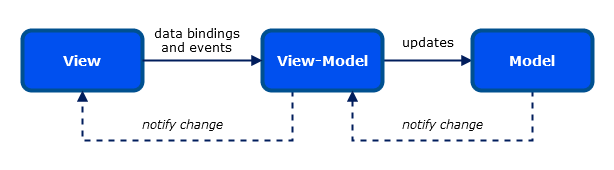
\includegraphics[width=\textwidth]{images/mvvm.png}
   \caption{\gls{mvvm} design pattern overview, adapted from \parencite[7]{microsoft_mvvm}}
   \label{fig:mvvm}
 \end{figure}

\subsection{View}
The view is what the user sees. It is responsible for the structure, layout and appearance of the application.
\subsection{View-Model}
The view model implements event handlers and properties, to which the view can bind to. It also notifies the view of any changes to the underlying data. It defines the functionality, offered by the \gls{ui}, but the view determines how it is presented. 
\subsection{Model}
The model encapsulates the data of the application and validation its logic.


\section{Vue.js}

Vue.js \parencite{vuejs_gh} is a progressive front end framework for building user interfaces and single-page applications based on the \gls{mvvm} design pattern described in \ref{sec:mvvm} \parencite{vuejs_book} \parencite{vuejs_guide}.  

\subsection{Components}
At the core of Vue.js are components, which are small, self-contained, composable and often reusable custom elements. Almost any type of application can be represented as a tree of components \parencite{vuejs_guide}. 

In more concrete terms, a Vue.js component is a single file with the extension of \code{.vue}, which consists of a \code{template}, \code{script} and optional \code{style} part. The \code{template} is a HTML-based template, which can be parsed by specification compliant browsers and HTML parsers. It can contain other components or html elements and is equivalent to the \textit{view} in \gls{mvvm}. 

The \textit{code} section of a Vue.js component includes the view-model of the component. Each component has a special JSON object \code{data}, equivalent to the \gls{mvvm} model.
The \code{script} part of a computed includes CSS-like styles.

\subsection{Data Binding}

Vue.js has built in support for \gls{databinding} using special directives.

\subsubsection{One-way Binding}
One-way binding is a one directional binding from source - a property of the model or other components to target - a property of a component or html tag. It can be achieved via the \code{v-bind} or \textit{moustache} syntax (double curly brackets). One-way bindings can also contain complex expressions.

\subsubsection{Two-way Binding}
Two-way binding is similar to one way-binding, but the value, which is bound to goes both ways and is synchronization. A typical example is a binding from an input field to a property of the model, e.g \code{email}. It can be achieved via the \code{v-model} binding directive.

\subsubsection{Event binding}
Event bindings are bindings of methods of the view model to events of components or html tags, for example the click on a button. It is done via the \code{v-on} or \code{@} directive. Event bindings could also contain anonymous methods.

\subsubsection{Computed Properties}
Computed properties are special properties, which can be used in \gls{databinding} and are a composition of other properties. 

\subsubsection{V-for Binding}
A \code{v-for} directive is a special type of binding used to render lists, which semantically can be used similarly to a \code{foreach} loop.

\section{ESLint}

ESLint \parencite{eslintMainPage} is a linting tool (linter) for ECMAScript/JavaScript. Linters are static code analysis tool, which can be used to flag and potentially automatically fix common code issues and enforce consistent code styling.

\subsection{Rules}
At the core of ESLint are rules. Rules are extensible pieces of code, bundled as plugins, which can be used to verify various aspects of code. An example would be a rule, which checks for matching closing parenthesis. 
Each rule consists of a \code{metadata} object
and a \code{create} function. The metadata object includes metadata such as documentation strings, the type of the rule and whether it is fixable or not.

Based on type, rules can be either \textit{suggestions}, \textit{problems} or \textit{layout}. Suggestions indicate some improvement, but are not required and would not cause the linting to fail. Problems on the other hand would result in a linting failure. Layouts are rules that care mainly about the formatting of code, such as whitespaces, semicolons, etc. 

If the fixable property is specified, it indicates that the errors reported by this rule can be automatically fixed. This can be applied via the \code{--fix} command line option. It has two possible values - \textit{code} or \textit{whitespace} indicating the type of fixes, that this rule would apply. For example in \glspl{ide} fixable \textit{code} errors would show a fix shortcut displayed next to them and \textit{whitespace} rules could be applied when saving the file.

The \code{create} function of rules takes as arguments a \code{context} and returns an object of methods which are called by ESLint for each node based on the \gls{visitor} pattern while traversing the \gls{ast}. 

\subsection{Selectors}
ESLint provides a very powerful matching mechanism for specifying what nodes to match called selectors \parencite{eslintSelectors} inspired by \textcite{estoolsEsQuery}.

Some selectors include:
\begin{itemize}
  \item AST Nodes - \code{MemberExpression} matches any node of type \code{MemberExpression}
  \item descendant -  \code{MemberExpression Identifier} matches any node of type \code{Identifier} who has a descendant of type \code{MemberExpression} in the tree
  \item child - \code{MemberExpression > Identifier} matches any node of type \code{Identifier} who has a direct parent (is a child of) of type \code{MemberExpression}
  \item :not -\code{:not(MemberExpression)} negation of a selector. In this case, matches any node, that is not a \code{MemberExpression} node
  \item :matches - \code{:matches(MemberExpression, Identifier)} matches any of the selectors. In this case, either a \code{MemberExpression} or \code{Identifier}.
  \item attributes - \code{Property[name=a]}. Matches any AST Node, whose specified attribute has the specified value.
\end{itemize}

\subsection{AST Explorer}
An incredibly useful tool when working with \glspl{ast} is \gls{ast} Explorer, developed by \textcite{astexplorer_fkling2021Jan}. It enables the exploration of syntax tree generated by various parsers and also includes the vue-eslint-parser \parencite{eslint_vue_parser}

\subsection{ESTree AST}
By default ESLint uses the \parencite{eslintEspree} parser to parse JavaScript source code into an \gls{ast} as defined by ESTree specification \parencite{estreeASTSpec}. When Parsing \textit{.vue} files ESLint uses this parser for the code inside the \code{<script>} tag.
  
\subsection{ESLint Parser Vue AST}

In order to parse the \code{<template>} section of \textit{.vue} files, ESLint uses the vue-eslint-parser \parencite{eslint_vue_parser}. This parser outputs an  \gls{ast} compliant with their own  \gls{ast}specification, defined in \parencite{eslint_vue_parser_ast}.

\chapter{Concept}
\label{chapter:concept}
\section{Parsing Vue.js}

\subsection{Assumptions}
It is assumed that the Vue.js code, for which interaction diagrams are going to be generated, compiles and does not contain syntactical errors. No checks are performed in order to verify that. Naturally, logical errors are not an issue.
\subsection{Limitations}
\label{concept:parsing_limits}

In order to be able to generate interaction diagrams, which capture every aspect of Vue.js, the generation must be directly based on an \gls{ast}, which covers every possible syntax, such as \cite{eslint_vue_parser}. 

The approach proposed here only includes the following features of Vue.js:
\begin{itemize}
    \item Event handlers (including anonymous method syntax and method reference syntax)
    \item Any one or two-way binding expressions (\code{v-model}, \code{v-bind}, "moustache", \code{v-if}) excluding \code{v-else}
    \item \code{v-for} statements for lists, excluding iterating through properties of an object or iteration with index (property zipped with index)
    \item distinguishing between properties and computed properties
    \item complex object and lists (non-nested) models 
    \item methods, including the resolution of arguments, they have been called with (excluding methods called with other methods as arguments)
\end{itemize}

\subsection{AST}

\begin{lstlisting}[style=antrl]
    grammar vue_simple;

    program: bindings methodDefinitions createdMethod topLevelProperties computedProperties;
    
    topLevelProperties: thisIdentifier*;
    methodDefinitions: methodDefinition*; 
    createdMethod: methodDefinition;
    computedProperties: (methodDefinitionIdentifier reads writes calls)*;
    
    methodDefinition: methodDefinitionIdentifier methodArgs reads writes calls;
    
    methodArgs: NAME_IDENTIFIER*;
    reads: accessedVariable*;
    writes: accessedVariable*;
    calls: calledMethod*;
    
    calledMethod: calledMethodIdentifier '(' calledArgs ')';
    accessedVariable: identifier;
    calledArgs: (calledMethod | accessedVariable)*;
    
    bindings: binding*;
    binding: tag bindingSource+;
    bindingSource: (accessedVariable | calledMethod) (EVENT_BINDING | ONE_WAY_BINDING)
                  | accessedVariable TWO_WAY_BINDING;
    
    tag: name tagId loc;
    tagId: LINE '_' COLUMN '_' LINE '_' COLUMN;
    name: UNICODE | identifier;
    loc: start end;
    start: LINE COLUMN;
    end: LINE COLUMN;
    
    calledMethodIdentifier: methodDefinitionIdentifier | id* NAME_IDENTIFIER;
    
    methodDefinitionIdentifier: THIS NAME_IDENTIFIER;
    thisIdentifier: THIS identifier;
    identifier: NAME_IDENTIFIER id*;
    
    
    id: NUMERIC_INDEX | GENERIC_INDEX | NAME_IDENTIFIER;
    
    //terminals, tokens
    LINE: [0-9]+;
    COLUMN: [0-9]+;
    
    EVENT_BINDING: 'event';
    TWO_WAY_BINDING: 'two-way';
    ONE_WAY_BINDING: 'one-way';
    
    GENERIC_INDEX: 'i' | 'j' | 'k' | 'l' | 'm' | 'n';
    THIS: 'this';
    
    NUMERIC_INDEX: [0-9]+;
    NAME_IDENTIFIER:  JS_IDENTIFIER;
    JS_IDENTIFIER:  (UNICODE | '$' | '_') (UNICODE | '$' | '_' | [0-9])*;
    UNICODE: [\u0000-\uFFFF];
\end{lstlisting}
\label{ast}

A Vue.js \gls{spa}, including all the necessary information for \ref{concept:parsing_limits}, can be defined using the above grammar. 

The application consists of \code{bindings} \code{methodDefinitions} a \code{createdMethod}, \code{topLevelProperties} and \code{computedProperties}. 

The \code{topLevelProperties} represent the \code{data} object of the Vue.js \code{script} tag. Each property will be represented flattened, as a list of identifiers and prefixed with \code{this},in order to indicate it belongs to the top level data object. For example \code{problem:\{a:0, b:0\}} will be represented as follows:

\begin{figure}[H]
    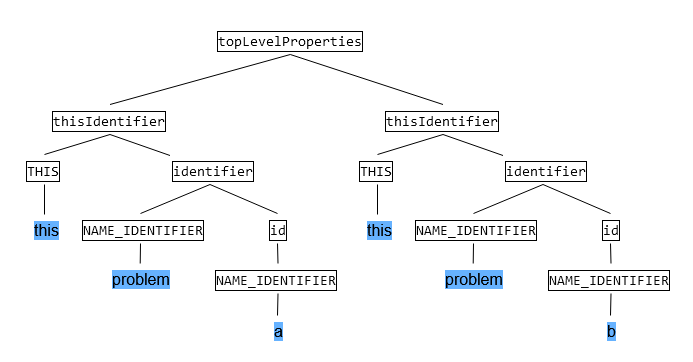
\includegraphics[width=0.8\textwidth]{images/ast_top_level.png}
     \caption{\gls{ast} for top-level example }
     \label{fig:ast_top_level}
\end{figure}

Bindings can be obtained from the Vue.js \code{template}.

Each binding consists of an HTML tag, an a list of binding sources for that tag - pairs of variable or method call and a binding type. The binding type represents the type of the binding - either event, one-way or two-way. Two-way bindings are only valid with properties, whereas for events and one-way bindings, both method calls and properties are possible, since in Vue.js a binding source could be an expressions defined as an inline anonymous functions (
    \code{<div v-if=\"value === true\"/>}
). The binding sources are a list, since a tag could have multiple different bound properties, or a bound expression. The information about how exactly the properties are bound, if it is the same type of binding, is discarded.

Method calls include the parameters they have been called with - other methods or just variables. It is also possible to call methods with binary expressions - those are represented as a special method, which takes 2 parameters - the left and right side operators of the binary expression. Expressions with multiple terms can be represented as multiple binary expressions. This representation loses information such as the order of operations, but since we are only interested in which properties are being accessed, this loss does not pose an issue.

A special case is accessing lists. For example \code{<div v-bind="problems[0].a"/>} would result in the following:

\begin{figure}[H]
    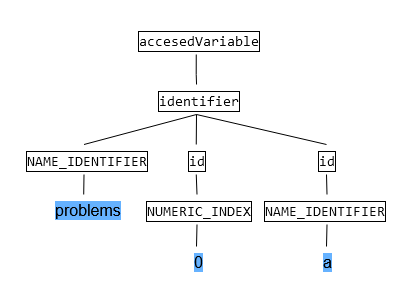
\includegraphics[width=0.8\textwidth]{images/ast_problems_0_a.png}
     \caption{\gls{ast} for example }
     \label{fig:ast_list_simple}
\end{figure}


\code{v-for} statements, are substituted:
\begin{lstlisting}[style=html]
<ul>
  <li v-for="subject in subjects" :key="subject.id">
    {{ subject.problems[0] }}
  </li>
</ul>
\end{lstlisting}
results in
\begin{lstlisting}[style=html]
subjects[i].problems[0]
\end{lstlisting}
which in term produces the following AST:

\begin{figure}[H]
    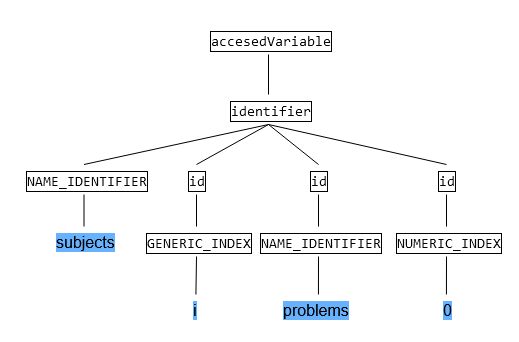
\includegraphics[width=0.8\textwidth]{images/ast_numeric_generic.png}
     \caption{\gls{ast} for example }
     \label{fig:ast_list_complex}
\end{figure}

Nested lists are also possible and would result in multiple generic indices being added.

Each tag includes its location in the source code (starting and ending line and column), which can also be used as an identifier. Tags also have humanly readable names, which are either equal to the the text of the tag, if it exists, or to the identifier of the first binding. 

\code{methodDefinitions} include all methods definitions from the \code{method} object of the \code{view-model}. Each method definition consists of the following
\begin{itemize}
    \item identifier - an identifier, equal to \code{this} followed by the name of the method
    \item arguments - names of arguments, each of which is a simple name identifiers
    \item reads - variable it reads from
    \item writes - variables it writes to
    \item calls - method calls, including arguments, same as for bindings 
\end{itemize}

\code{computedProperties} are similar to \code{methodDefinitions} with the exception that they do not have arguments. Albeit bad practice, it is still possible for computed properties to have side effects and therefore they were modelled as methods.

%%%%%%%%%%%%%%%%%%%%%%%%%%%%%%%%%%%%%
%                                   %
%   Interaction Diagram Generation  %
%                                   %
%%%%%%%%%%%%%%%%%%%%%%%%%%%%%%%%%%%%%
\section{Interaction Diagram Generation}

The simplified Vue.js \gls{ast} can be used to create a directed graph, which will represent the interaction diagrams. It is hard to directly generate this graph, therefore the capabilities of a directed, compounded graph will be leveraged and later on converted to a directed graph. 

Vertices in this graph have the following properties
\label{concept:interaction_diagram_structure}
\begin{enumerate}
    \item \gls{guid} - used to reference and globally identify the vertex 
    \item \code{label} - the name of the vertex, which is going to be displayed
    \item \code{type} - the type of the vertex (data, tag or method). Additionally for data vertices: numeric, generic or undefined (representing simple data vertices)
    \item \code{loc} - defined only on tag vertices. Their location in the source code
    \item \code{parent} - defined only on vertices of type 'data'. A \gls{guid} of another vertex, used for a child/parent relationship (compound graph).
\end{enumerate}

Edges in the graph are directed and each have a label property, which is one of 'event', 'calls' or 'simple'. 

The core idea of the algorithm is to generate vertices only for nodes which are being accessed instead of the whole application. A second pass of the data is also needed to add additional edges for lists. 

\subsection{Variable Identifiers}
\label{concept:variable_identifiers}
Variable identifiers are represented by \astnode{identifier} and \astnode{thisIdentifier} in the \gls{ast} \ref{ast}. For the \astnode{this} and for each \astnode{id} node in the \astnode{identifier} or \astnode{thisIdentifier} a vertex is created in order. 
Those vertices are connected using unidirectional edges, labeled with 'data' and also each vertex (excluding the first one) has its parent set to the previous. There is one exception to this process - When accessed from \astnode{write} of a \code{method}, nodes of type \astnode{GENERIC_INDEX} are omitted. The reason behind this will be explained in this section \ref{concept:why_create_list};


Each vertex has a \gls{guid} equal to the value of its terminal symbol (\astnode{NUMERIC_INDEX}, \astnode{GENERIC_INDEX} or \astnode{NAME_IDENTIFIER}), concatenated with the value of the previous vertex.
The \code{label} of those vertices are equal to the terminal symbol in case of \astnode{NAME_IDENTIFIER} and in case of \astnode{GENERIC_INDEX} and \astnode{NUMERIC_INDEX}, combined with the \code{label} of the previous vertex using square braces. Set the type of each vertex to 'data'. Add the type 'numeric' to vertices created from \astnode{NUMERIC_INDEX} nodes and 'generic' to vertices created from \astnode{GENERIC_INDEX} nodes. 

\begin{figure}[H]
    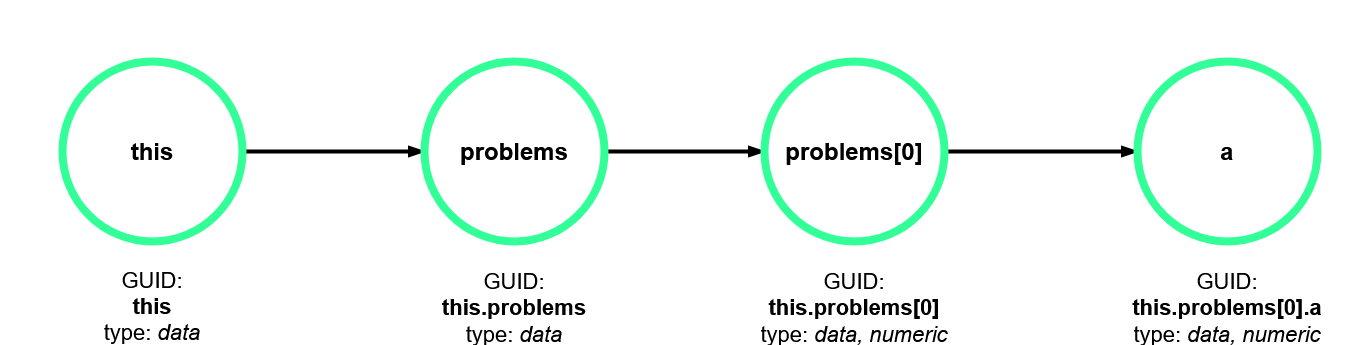
\includegraphics[width=0.8\textwidth]{images/graph_simple.png}
     \caption{Example Graph obtained for the identifier \code{this.problems[0].a} }
     \label{fig:graph_simple}
\end{figure}

\subsection{Object representation}

Using the representation for identifiers in the previous section, objects will result in being displayed dynamically, based on which properties are accessed. Nodes and edges are created on a 'create if non-existent' basis. In the example below, if \code{this.problem.b} is accessed after \code{this.problem.a} it will only result in the creation of the node \code{a} and edge \code{this.problem} -> \code{this.problem.b}.

\begin{figure}[H]
    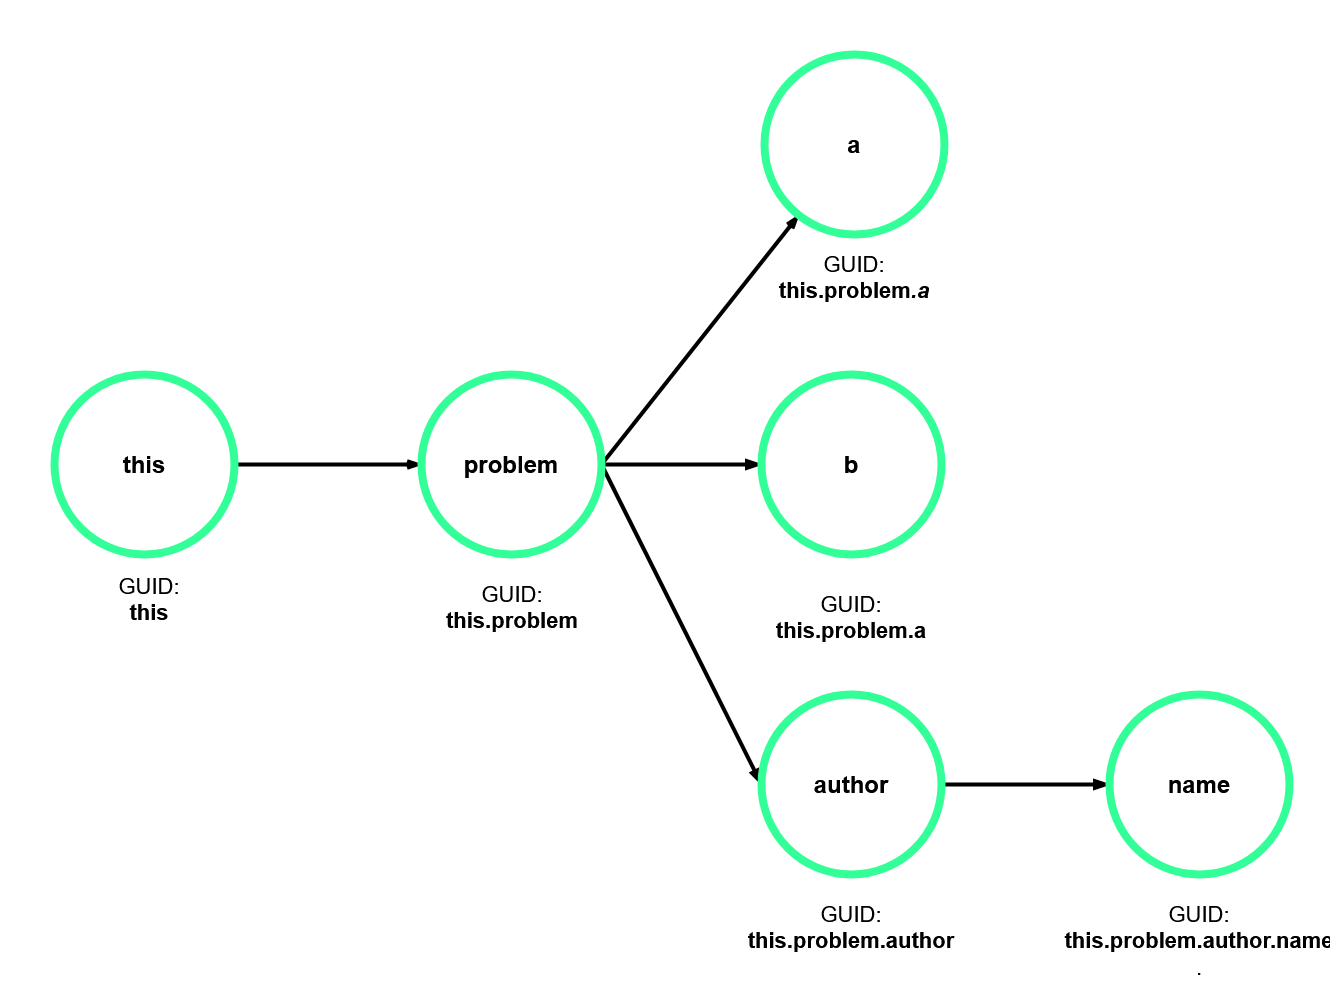
\includegraphics[width=0.8\textwidth]{images/graph_object.png}
     \caption{Example Graph for the following object accesses - \code{this.problem.a}, \code{this.problem.b},  \code{this.problem.author.name} }
     \label{fig:graph_object}
\end{figure}

Furthermore, updates can be formulated nicely with the above representation. If \code{problem} were to be changed, it would result in a cascade update of all properties. If \code{author} would be change, it would only result in a cascading change in \code{name}. 

\subsection{List representation}
\label{concept:list_creation}

Lists will be represented based on the template in \ref{fig:graph_list_generic} for a list named $P$.  %TODO for a list named $P$ don\tlike this
\begin{figure}[H]
    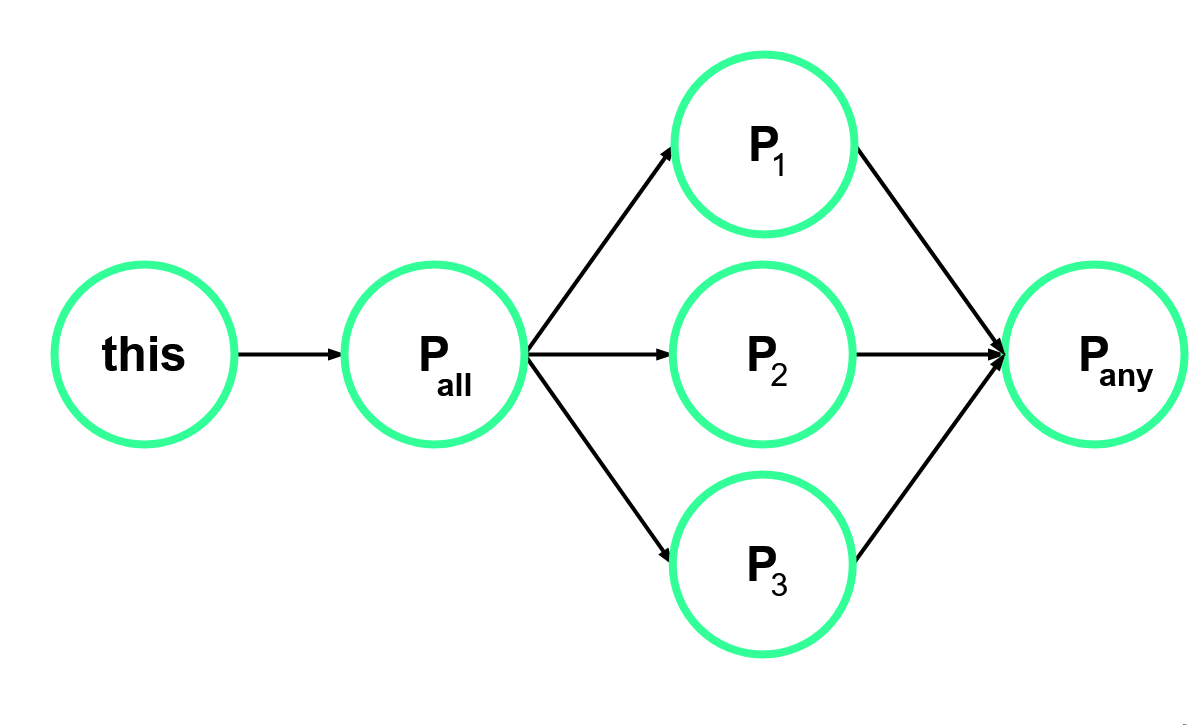
\includegraphics[width=0.8\textwidth]{images/graph_list_generic.png}
     \caption{Generic List representation}
     \label{fig:graph_list_generic}
\end{figure}

Concrete elements, which are accessed, are denoted as $P_{<index>}$ and additionally a vertex $P_{all}$, which can be used to update all elements of a list\label{concept:why_create_list} and their properties, is created. Another vertex $P_{any}$ is also created, which can be used to observe once any vertex of $P_1$, $P_2$, $P_3$, \dots $P_n$ changes. If $P_1$ were to be updated by any method, it would not result in updates to any of $P_2$, $P_3$, \dots $P_n$

The same construct can also be leveraged when it comes to properties of list elements. Each top level property of that element will have an $all$ vertex, connected to the $P_{all}$ node of the list.  

\begin{figure}[H]
    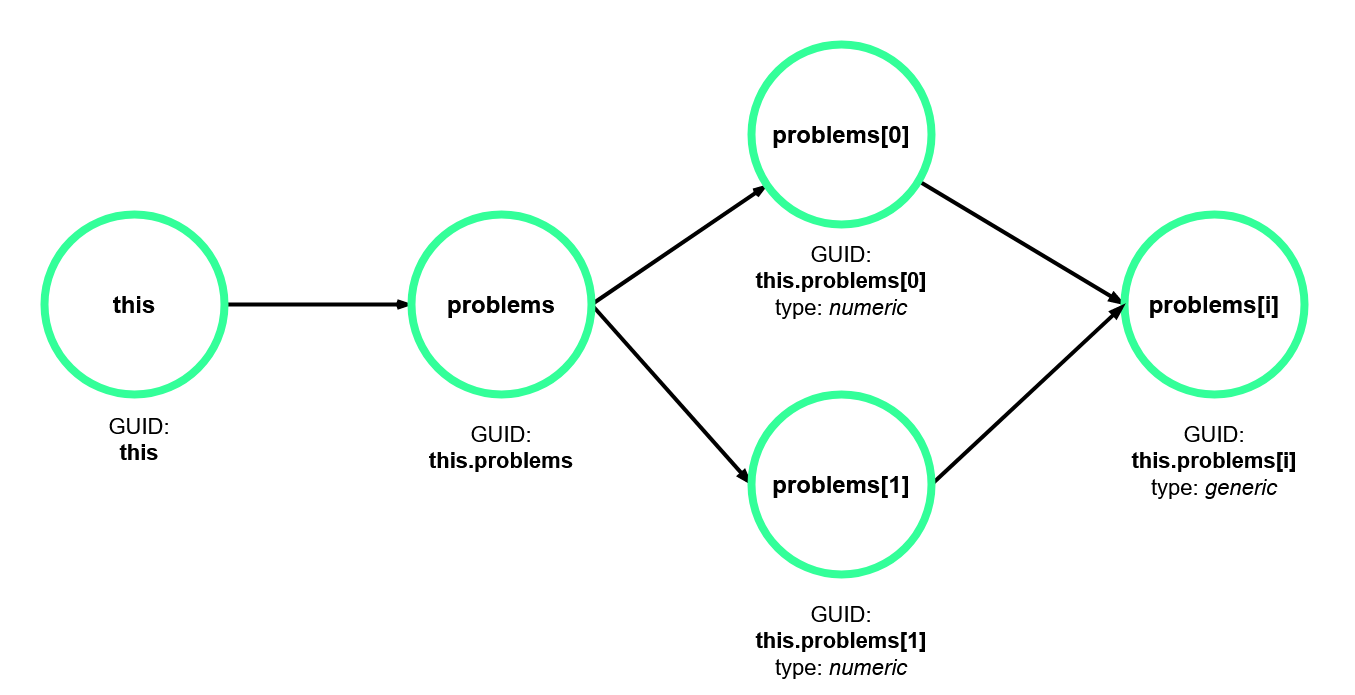
\includegraphics[width=0.8\textwidth]{images/graph_list.png}
     \caption{Concrete example of a list representation}
     \label{fig:graph_list}
\end{figure}

\subsection{Method representation}
\label{concept:methods}
Methods have two related \gls{ast} nodes - \astnode{methodDefinition}, representing the definition of a method and \astnode{calledMethod} representing a call of a method. 

First it should be determined if a vertex needs to be created for an \astnode{calledMethod} node. This is done by looking up based on the name of the \astnode{calledMethod} in \astnode{methodDefinition}, ignoring \astnode{THIS}. If the lookup is successful a vertex should be created as described below. If not, it should be checked if the method is a method call on a top level property instance. This can be done by comparing if it starts in the same way as one of \code{topLevelProperties}. %TODO that's not so clear an a bit slapped here. check tomorrow
If that's the case, it is assumed, that it mutates whole property and the method should instead be treated as a write operation.
If both of the above fail, the called method does not belong to context and is of no interest.

The next step is to resolve the names of the arguments it has been called with \astnode{calledArgs}. Every argument, that can neither be found in \astnode{computedProperties} nor \astnode{topLevelProperties} is replace by a fixed word such as $OTHER$ or $*$. In order to obtain the \gls{guid} of the vertex, the name of the \astnode{methodDefinitionIdentifier} is taken, \astnode{THIS} is excluded, and concatenated with the the resolved arguments, which are joined with $,$ and surrounded with brackets. The \code{label} of this node is equal to its name, excluding \astnode{THIS} from arguments. 

The vertex for the method call is now completed. Multiple calls of this method with the same arguments will all result in the same vertex.

Now vertices for nodes the method interacts with, based on its \astnode{methodDefinition}, have to be created. Those include the variables it reads - \astnode{reads}, and writes - \astnode{writes} and methods it calls - \astnode{calls}. 

Firstly, the arguments from the \astnode{methodDefinition} need to be substituted with the resolved arguments the method was actually called with and update all \astnode{reads}, \astnode{writes}  \astnode{calls} referencing them. All of them, which do not start with \astnode{THIS} can be discarded, since they do not belong to the context. Once filtered out, create a list of vertices for each variable in \astnode{reads} and \astnode{writes} as described in \ref{concept:variable_identifiers} and connect the most precise of those (the last of each list) to the method vertex. For the vertices resulting from \astnode{writes}, this edge has a label of 'writes' and the property vertex as the source and method vertex as the sink. For the vertices resulting from \astnode{reads}, this edge has the method vertex as the source and property vertex as the sink. 
Finally the process described in this section is repeated recursively for each \astnode{calledMethod} node in \astnode{calls} and an edge labeled 'calls' is added from the current method vertex to the resulting ones. 

\subsubsection{Computed property representation}
\label{concept:computed_property}

Computed properties are represented similarly to methods, except they cannot have arguments, so no substitution of arguments is required. When defining their \code{label} and \gls{guid} both are equal to the \astnode{methodDefinitionIdentifier}. \astnode{reads}, \astnode{writes} and \astnode{calls} are computed in the same manner as methods. 

\subsubsection{Combining it all together}
\label{concept:algorithm_create_diagrams}

Interaction diagrams can be generated from the simplified Vue.js \gls{ast} in the following way:

%TODO how to indent
For each \astnode{binding} in \astnode{bindings}:
- for each \astnode{tag}, \astnode{bindingSource}  in \astnode{binding}:

Create a vertex for \astnode{tag}, with a \gls{guid} \astnode{tagId} and label \astnode{name} and type 'tag'.

if the \astnode{binding} is an \astnode{accessedVariable}, determine if it is a computed property by looking it up in \astnode{computedProperties} and if so, treat it as a computed property, and create vertices as described in \ref{concept:computed_property}. Otherwise determine if it as top level property, by doing a lookup on \astnode{topLevelProperties}, treat it as a property and create vertices for it as described in \ref{concept:variable_identifiers}. In either cases, connect it to the \astnode{tag} vertex, based on the binding type. If the \astnode{accessedVariable} is neither, it does not belong to context and can be discarded. %TODO YADA YADA, ignore this prefix when checking

if the \astnode{binding} is an \astnode{calledMethod} create a vertices for it as described in \ref{concept:methods}. Connect it to the \astnode{tag} vertex, based on the binding type.

Based on binding type, the following edges are created:
A) If the binding type is an event binding, create an 
edge with the tag vertex as a source and the binding vertex as sink and label it 'event'. 
B) If the binding type is one-way, create an edge with the binding vertex as source and the tag vertex as sink.
C) If the binding type is two-way, create both edges - A) and B).

For the initial method - \astnode{createdMethod}, create a vertex with \gls{guid} and name equal to \textit{created} and create vertices for its \astnode{reads}, \astnode{writes} and \astnode{calls} analogous to methods as described in \ref{concept:methods}. 


Once all of the above is done, additional edges will need to be added for the \textit{all} vertices of properties of elements inside lists \ref{concept:list_creation}. Also the edges to the \textit{any} vertex will be missing. 

'numeric' vertices to the 'generic' one. 

This is achievable by first finding all vertices of type 'generic' or 'numeric' and obtaining the parent of each of them. Those parents form a subset of all vertices, that have have 'generic' or 'numeric' vertices as children and additionally other properties (properties on list elements, with $type(v) \neq generic, type(v) \neq numeric$). 
For each of those parent vertices $p$:
Firstly, connect each 'numeric' vertex to the 'generic' one. Recursively connect each child in the tree of the 'numeric' vertex to the child of the tree of the 'generic' vertex with the same name. If either does not exist, no edge is created. Do the same for $p$ and all 'numeric' vertices and the 'generic' vertex.

\begin{figure}[H]
    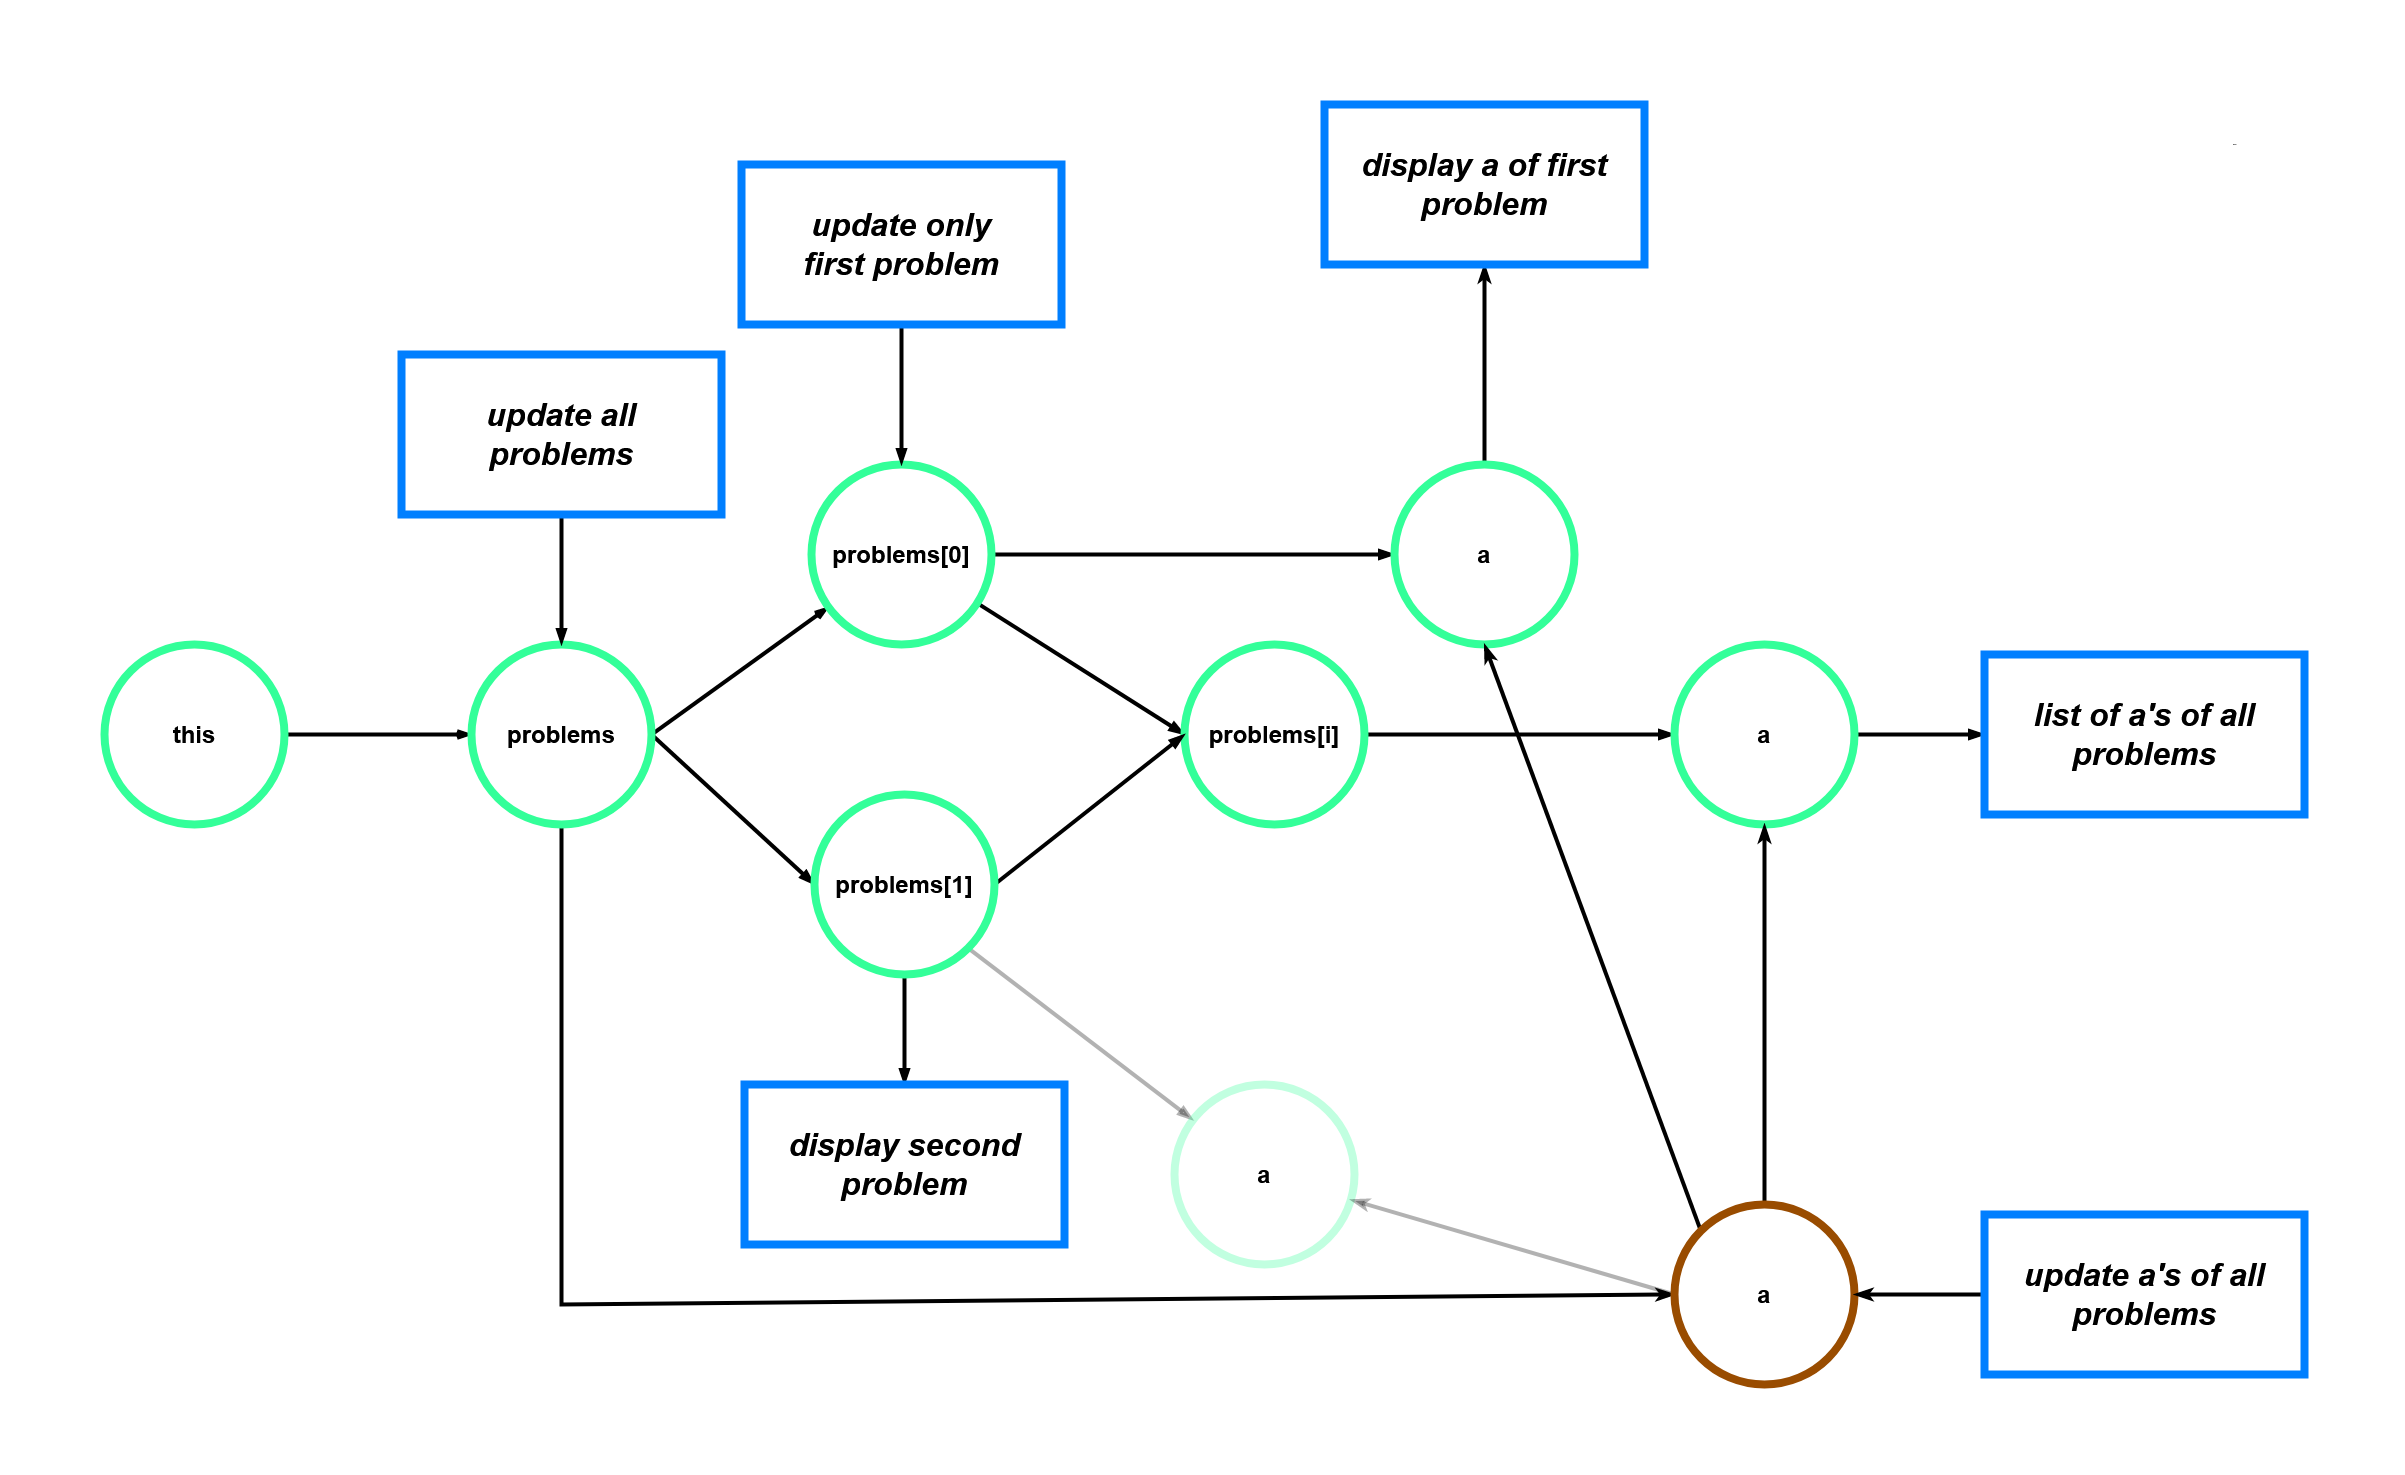
\includegraphics[width=0.8\textwidth]{images/graph_complete_example.png}
     \caption{Example Graph including list elements with properties}
     \label{fig:graph_complete_example}
\end{figure}

%TODO describe this and also verify above
\section{Scenario Generation}
\label{concept:scenario_generation}
In order to generate scenarios in Gherkin, interactions can be sliced in a similar manner as described by \textcite{zhang2019scenario} and summarized in \ref{intro:zhang_interaction_diagrams}.

Let $N$ denote the set of all nodes in the graph and $E$ denote all edges in the graph. Let $n \in N$, $m \in N$ be any two nodes in the graph and $(n, m) \in E $ represent an edge from $n$ to $m$. Let $type(n)$ be a function, that returns the type of a node and $label(n, m)$ be a function that returns the label of the edge from $n$ to $m$. Let $E_{out}(n)$ be a function, which returns all outgoing edges of $n$.
Let $E_{in}(n)$ be a function, which returns all incoming edges to $n$.

Let $N_I$ denote all nodes, that the user can interact with. A node $n \in N$ is also in $N_I$ if $\exists e \in E_{out}(n)$ where $label(e) = event$. Let $N_H$ denote all html tag nodes. A node $n \in N$ is also in $N_H$ if $type(n) = tag$. 
Given a node $n_H \in N_H \cup {created}$, a node $m_H \in N_H$ reacts to $n_H$ iff
\begin{enumerate}
    \item $\exists n_0,n_1,n_2, \ldots,n_k \in N, n_0=n_H,n_k=m_H$ such that for each $0 \leq i < k  $ $(n_i,n_{i+1}) \in E$, and $label(n_i,n_{i+1})\neq event$ and if $label(n_i,n_{i+1}) \neq calls$ $\forall n_{i+1_{in}} E_{in}(n_{i+1})$ $label(n_{i+1_{in}}) \neq event$ 
\end{enumerate}

Analogous to \cite{zhang2019scenario} let $l(n)$ denotes all nodes, that react to $n$. A sequence of user interactions, starting with the initial function is referred to as a \textit{scenario} $A=(a_0,a_1,\ldots, a_n)$ where $a_0=created$ and $\forall0 < k \leq n, a_k \in N_I$. 
Define the HTML tags, to which a scenario reacts, to be equal to the tags to which the last tag in the scenario reacts $l(A)=l(a_n)$. Define a function that returns the last element in a scenario - $last(A) = a_n$

The set of scenarios is generated by starting with the initial scenario, containing only the initial function $S_0 = \{(created)\}$. It is then prolonged by all tags $n \in N_I$, representing that the user can click anywhere. For further steps, only tags, that can be updated are included, so additionally $n \in l(A)$ must hold. The newly included tag should also not be the same as the last element of the scenario, which means that also $n \neq last(A)$ must hold.
Formally:
Define $A \oplus x = a_0,a_1,\ldots,a_n,x$. Then
\begin{align}
    S_n = \begin{cases} 
        \{(created)\} &\mbox{if } n = 0 \\
        \{ p \oplus x |p \in S_{n-1}, x \in \mathcal{I}\} &\mbox{if } n = 1 \\
        \{ p \oplus x |p \in S_{n-1}, x \in l(p) \cap \mathcal{I}, x \neq last(p) \} 
    \end{cases}
\end{align}
This is repeated up to $k$ times, where $k$ is a constant set by the user. 

A Gherkin scenarios templated can then be obtained by the following template:

Scenario - $n_0,n_1 \ldots n_k$

Given - $n_0, n_1 \ldots n_{k-1}$

When - $n_k$

Then - $l(n_k)$


%TODO dynamically and then connect idea

%lists better explain, generic acts as the any, etc.

\chapter{Implementation}
\label{chapter:implementation}
\section{Project Structure and Overview}
The application is written mostly in TypeScript using npm as a package manager and Node.js as a runtime environment. 




%TODO eslint only js thats why no ts. at intro probably
Notable dependencies are TypeScript, for stricter syntax and types, lodash\parencite{lodash} for enrichening of collections, graphlib\parencite{graphlib} for the interaction diagrams graph,  babel\parencite{babel} as a transcompiler, eslint\parencite{eslintMainPage}, estree\parencite{estreeASTSpec} and eslint-plugin-vue\parencite{eslint_vue_parser} for parsing Vue.js code, d3-graphviz\parencite{graph_viz} in comination with light-server\parencite{light_server} for visualization of the generated interaction diagrams. The full list of dependencies can be found in the \code{package.json} of the project.
%TODO cite all of those directly?

%lint, ci, tests, etc? gith?

\subsection{Project structure}
%TODO define lang
The main source files of the project and their tests are included in the \code{src} directory and structured in several packages, each corresponding to a step in the process, except common, which is shared among all steps. Each will be described in more detail in the following sections.
Each package includes a models directory, which inludes the data types defined and used in this section.
The \code{web} directory contains code used to view the resulting diagram in the browser.
The \code{scripts} directory includes helper bash scripts, \code{results} holds snapshots of the results throughout development (with the latest being the current) and \code{resources} hold various additional files needed.
\begin{lstlisting}
  root:.
  |-- resources
  |   |-- output
  |
  |-- results
  |
  |-- scripts
  |
  |-- src
  |   |-- common
  |   |   |-- models
  |   |
  |   |-- main.ts
  |   |
  |   |-- generator
  |   |   |-- models
  |   |
  |   |-- parsing
  |   |   |-- builders
  |   |   |-- models
  |   |   |-- visitors
  |   |
  |   |-- scenarios
  |
  |-- web
\end{lstlisting}

\section{Parsing Vue.js}

Instead of implementing a parser, which directly outputs the simplfied Vue.js \gls{ast} described in \ref{ast} the capabilities of \textcite{eslintMainPage}  %TODO add cit
and \parencite{eslint_vue_parser} were used. 
The source files, which handle the parsing reside in the \code{parsing} directory.
The \code{ESLinter} class provides a wrapper around the Node.js API of ESlint. Custom visitors are implemented in order to extract the necessary nodes from the \gls{ast} of ESLint. Each visitor has a matching file in \code{models}, which holds the models specific to that visitor, and a \code{builder}, which keeps track of the visited nodes and builds the result data type. There are a total of three visitors - one for top level properties, another for bindings and the last one for method defintions, computed properties and the created method.
 
\subsection{Common Data Types}
Below are the common data types used by all visitors.
\begin{lstlisting}
export type Identifier = This | NameIdentifier | NumericIndex 
| GenericIndex;

interface BaseIdentifier {
  readonly name: string;
}
export interface This extends BaseIdentifier {
  name: "this";
  discriminator: IdentifierType.THIS;
}
export interface NumericIndex extends BaseIdentifier {
  discriminator: IdentifierType.NUMERIC_INDEX;
}
export interface GenericIndex extends BaseIdentifier {
  discriminator: IdentifierType.GENERIC_INDEX;
}
export interface NameIdentifier extends BaseIdentifier {
  discriminator: IdentifierType.NAME_IDENTIFIER;
}
\end{lstlisting}

%TODO lang
\begin{lstlisting} 
export type Entity = Method | Property;

export interface Property {
  id: Identifiers;
  discriminator: EntityType.PROPERTY;
}
export interface Method {
  id: Identifiers;
  args: ReadonlyArray<Entity>;
  discriminator: EntityType.METHOD;
}
\end{lstlisting}
Discriminators are used to be able to diferentiate between the types using type guards. The enums themselves are omitted here (\code{IdentifierType}, \code{EntityType}). The definitions here are not exactly the same as in the \gls{ast} \ref{ast} - some constraints are omitted, such as method names having to end on a a \code{NameIdentifier}. This will be given, since the parsed code would be invalid javascript otherwise.
\subsection{Top Level Properties}
The result of the top level properties has the following data type.
\begin{lstlisting}
export type TopLevelProperties = Array<Property>;

export interface TopLevelPropertiesResult {
  topLevel: TopLevelProperties;
}
\end{lstlisting}

The top level properties visitor is the simplest of all since it only reacts to the top level \code{data} node inside the \code{script} object  of the Vue.js \gls{spa}, which is a \code{ObjectExpression} \ref{eslint:object_expression}. It can be selected via the following selector:

%TODO lang
\label{impl:top_level_select}
\begin{lstlisting}

"ExportDefaultDeclaration > ObjectExpression > 
Property[key.name = data] ReturnStatement > ObjectExpression"(node){
  ...
}
\end{lstlisting}
In natural language the selector reads: "Select ObjectExpression nodes, which have a direct parent ReturnStatement, that has an indirect parent Property with a property \code{key.name} equal to \code{data} and a direct parent ObjectExpression with a direct parent ExportDefaultDeclaration.

For each of the properties \ref{eslint:property} of the \code{ObjectExpression} the name of the key (identifier) is stored. If the property is an object (value of \code{ObjectExpression} \ref{eslint:object_expression}) it is concatenated with the previously obtained key. Finally all obtained properties are prefixed with 'this'.

\subsection{Bindings}
The result of the bindings visitor has the following data type.
\begin{lstlisting}
  export enum BindingType {
    EVENT = "event", ONE_WAY = "one-way", TWO_WAY = "two-way",
  }
  
  export interface Tag {
    id: string;
    loc: Location;
    name: string;
    position?: string;
  }
  
  export interface BindingValue {
    item: Entity;
    bindingType: BindingType;
  }
  
  export type Binding = { tag: Tag; values: BindingValue[] };
  export interface BindingsResult {
    bindings: Binding[];
  }
\end{lstlisting}

The ESlint \gls{ast} nodes, which are interesting when parsing the bindings are \code{VElement} \ref{eslint:velement}, 
\code{Identifier} \ref{eslint:identifier}, \code{MemberExpression} \ref{eslint:member_expression} and \code{CallExpression} \ref{eslint:call_expression}. 

A \astnode{identifier} \ref{ast}, abstracted
in \code[]{common/identifier.ts}  can be a single \code{Identifier} or a \code{MemberExpression}, which can contain other \code{Identifier} nodes or \code{MemberExpression} nodes. Property Identifiers are extracted by finding the root \code{MemberExpression} or \code{Identifier} and traversing it. It is easy to determine if a \code{MemberExpression} or \code{Identifier} is the root - its parent is anything but a \code{MemberExpression}.

A \code{CallExpression} contains information about the name of the method and the arguments it has been called with, both in the form of nested \code{MemberExpression} and \code{CallExpression} nodes. Once again, only the root \code{CallExpression} node is extracted and converted to a \astnode{calledMethod} \ref{ast}, abstracted in the \code{Method} interface in \code{shared.ts}.

\code{VElement} nodes represent any HTML tag, matching a \astnode{tag} \ref{ast} abstracted in the \code{Tag} interface in code{template-bindings.ts} and contain information about the location of the tag and potentially a \code{VText} \ref{eslint:vtext} node, which will be set as its name if it is present. If not present, the name of the tag is equal to the name of the first binding. Therefore, information about tags is extracted once a \code{VELement} is exited, since all bindings will be known at this point.

Further, the binding type has to be determined. This can be extracted based on the \code{VAttribute} \ref{eslint:VAttribute}. Event bindings have a \code{VAttribute} with a \code{key.name.name} equal to 'on', two-way bindings equal to 'model' and everything else is interpreted as one-way bindings. This includes moustache statements, \code{v-bind}, \code{v-if} bindings and all other except \code{v-for} statements. This filter be achieved via the powerful \code{:not} in combination with \code{:matches} selectors: 
%TODO lang
\begin{lstlisting}
:not(:matches(
  VAttribute[key.name.name=on], 
  VAttribute[key.name.name=model],
  VAttribute[key.argument.name=key],
  VAttribute[key.name.name=for]))
\end{lstlisting}

With all the above, for example to match all two-way bindings and pass them on to the builder can be done via 
\begin{lstlisting}
  
"VAttribute[key.name.name=model] > VExpressionContainer
:matches(MemberExpression, Identifier, CallExpression)"(
  node) {
  if (utils.isRootNameOrCallExpression(node) && 
  utils.notArgument(node))
    builder.identifierOrExpressionNew(node, BindingType.TWO_WAY);
},
\end{lstlisting}

%TODO note why not args - method knows exactly what part

Bindings also need to substitute \code{v-for} statements. This is done by substituting the left side of the \code{v-for} statement with its right side and a generic index in all bindings that use it.

\subsection{Method Definitions}

\begin{lstlisting}
export interface MethodDefinition {
  id: Identifiers;
  args: ReadonlyArray<Property>;
  reads: ReadonlyArray<Property>;
  writes: ReadonlyArray<Property>;
  calls: ReadonlyArray<Method>;
}
export type MethodDefinitions = Array<MethodDefinition>;

export interface MethodsResult {
  init?: MethodDefinition;
  computed: MethodDefinitions;
  methods: MethodDefinitions;
}
\end{lstlisting}
All method definition like structures (computed properties, created) and methods are parsed by the visitor defined in \code{methods.js}.
Analogous to how the top level \code{data} object is selected \ref{impl:top_level_select}, the \code{methods}, \code{created} and \code{computed} objects can be selected. 
The name of the method including its arguments can be extracted from by \code{Property[value.type=FunctionExpression]} nodes. Using this information, one can have three selectors, one of each type, to determine what is being defined. For example for regular methods:
 
\begin{lstlisting}

"ExportDefaultDeclaration > ObjectExpression > Property
[key.name = methods] Property[value.type=FunctionExpression]"(node) {
  builder.newMethod(node, MethodType.METHOD);
},
\end{lstlisting}

Further the properties read, written and methods called need to be extracted. Methods called can be obtained by selecting \code{CallExpression} nodes. Properties written to can be obtained from the left side of a \code{AssignmentExpression} \ref{eslint:AssignmentExpression}.
There does not seem be an easy way to select all properties read from. Therefore all accesed identifiers are first stored and everything except reads, that can have an identifier (object properties, variable declarations, variables written to and names of called methods) is subtracted from it, in order to obtain the variables that the method reads from.

The following code can be used to obtain all variables written to by the current method-like in scope. 
\begin{lstlisting}
"ExportDefaultDeclaration > ObjectExpression > 
:matches(Property[key.name = methods], Property[key.name = created],
Property[key.name = computed]) AssignmentExpression"(node) {
  builder.identifierOrExpressionNew(node.left, AccessType.WRITES);
},
\end{lstlisting}
\subsection{Output}
Combinging all of the above, the following data structure is output.
\begin{lstlisting}
export class Result {
  fileName: string;
  topLevel: TopLevelPropertiesResult;
  methods: MethodsResult;
  bindings: BindingsResult;
  ...
}
\end{lstlisting}
\label{impl:result}
\section{Interaction Diagram Generation}
The generation of the interaction diagram graph from the result class from \ref{impl:result} is done in the \code{Transformer} class. 

The resolution of methods is abstracted in the \code{MethodResolver} class. It produces a 
\code{ResolvedMethodDefintition} for each called method in bindings and the initial method. In order to prevent duplicate resolution of methods and wasting of resources a \code{MethodCache} is introduced. The \code{Transformer} does not use the \code{MethodResolver} directly, but instead accesses it via the \code{MethodCache}. The cache includes directly called (bound to) and indirectly called (calls of methods), for each of which vertices will have to be created. 
Each \code{ResolvedMethodDefintition} has the following data type:
\begin{lstlisting}
export enum GeneralisedArgument {
  METHOD = "method",OTHER = "other",
}
export type ResolvedArgument =
  | Property | GeneralisedArgument.METHOD | GeneralisedArgument.OTHER;
export interface ResolvedMethodDefintition {
  id: Identifiers;
  args: ReadonlyArray<ResolvedArgument>;
  reads: ReadonlyArray<Property>;
  writes: ReadonlyArray<Property>;
  calls: ReadonlyArray<CalledMethod>;
}
export interface CalledMethod {
  id: Identifiers;
  args: ReadonlyArray<ResolvedArgument>;
}
\end{lstlisting}


As the underlying structure for the graph graphlib is used and wrapped in an own class - \code{ExtendedGraph}. It creates vertices on a 'create if not exist' basis by first looking up to see if the vertex exists in the graph, and if it does, does not add it again. Presence of edges is not checked, if an edge is added again, the previous one is simply overwritten. There can only be one edge per direction between two nodes, since no multigraph is used. Nodes and Edges in the graph have the following structure, as specified in \ref{concept:interaction_diagram_structure}:

%TODO format
\begin{lstlisting}
export enum EdgeType {
  SIMPLE = "simple", EVENT = "event", CALLS = "calls",
}
export interface Edge {
  source: Node;
  sink: Node;
  label: EdgeType;
}
\end{lstlisting}
\begin{lstlisting}
export enum NodeType {
  TAG = "tag",  DATA = "data", METHOD = "method", INIT = "init",
}

export type Node = TagNode | DataNode | MethodNode | InitNode;
interface BaseNode {
  id: string;
  name: string;
}
export interface TagNode extends BaseNode {
  loc: Location;
  discriminator: NodeType.TAG;
}
export interface MethodNode extends BaseNode {
  discriminator: NodeType.METHOD;
}
export interface InitNode extends BaseNode {
  discriminator: NodeType.INIT;
}
export interface DataNode extends BaseNode {
  parent?: string;
  type: IdentifierType;
  discriminator: NodeType.DATA;
}
\end{lstlisting}


The algorithm for generating the interaction diagrams graph as described in \ref{concept:algorithm_create_diagrams}
is implemented in the \code{Transformer} class.

First the init method is resolved by querying the \code{MethodCache} and afterwards each of the bindings. The order is not important. If the bindings are properties, the vertices for them are created directly. If they are methods or computed properties, they are resolved by the \code{MethodCache} and the correct edges based on the binding type created. The above is done in the \code{addInit()} and \code{addBindings()} methods.

At this stage no vertices are created for the reads, writes, and calls properties of the resolved methods. 
This happens in the \code{addIndirectlyCalledMethods()} method, after all bindings and the init method have been resolved by taking all methods stored in the \code{MethodCache} and creating the appropriate vertices.

Lastly in the \code{addEdgesForLists} method additional edges will be added for the \textit{all} vertices of properties of elements inside lists.

\section{Scenario Generation}
The scenario generation is implemented in the \code{scenario.ts} file and currently ouputs the obtained scenarios, tags, nodes react to and the gherkin scenarios templates to the console.

\section{Usage}


\chapter{Evaluation}
\label{chapter:testing_and_evaluation}
\section{Math for Kids - Simple Properties}
\textcite{zhang2019scenario} use an example of a small \gls{spa} titled "Math for kids", which generates simple math addition problems and keeps track of a small statistic, which includes the number of correctly and incorrectly answered problems. The same application has been implemented and extended in Vue.js and will be used to display the capabilities of the interaction diagram and scenario generation application.

\begin{figure}[H]
    \centering
    \begin{subfigure}[b]{0.45\textwidth}
         \centering
         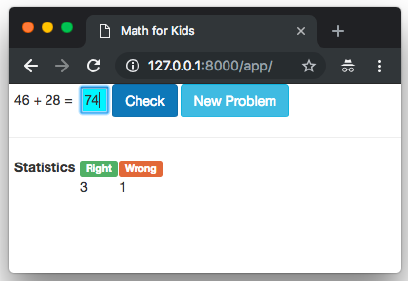
\includegraphics[width=0.45\textwidth]{images/math_for_kids_zhang.png}
         \caption{Math for Kids in AngularJS by \textcite{zhang2019scenario}}
    \end{subfigure}\hfill%
    \begin{subfigure}[b]{0.45\textwidth}
        \centering
        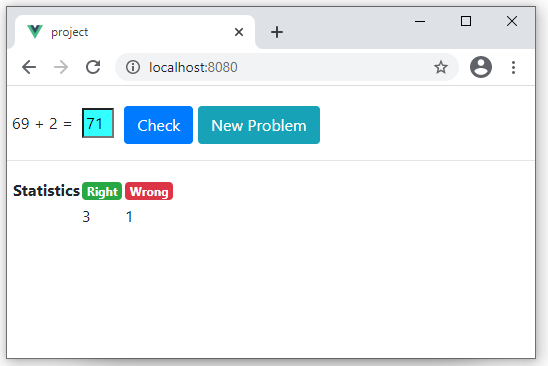
\includegraphics[width=0.45\textwidth]{images/math_for_kids_own.png}
        \caption{Own implementation of Math for Kids in Vue.js}
    \end{subfigure}
\end{figure}

The source code can be found in \code{resources/test-files/test.vue} and also in \ref{appendix:math_kids_basic_source_code}.
\begin{figure}[H]
    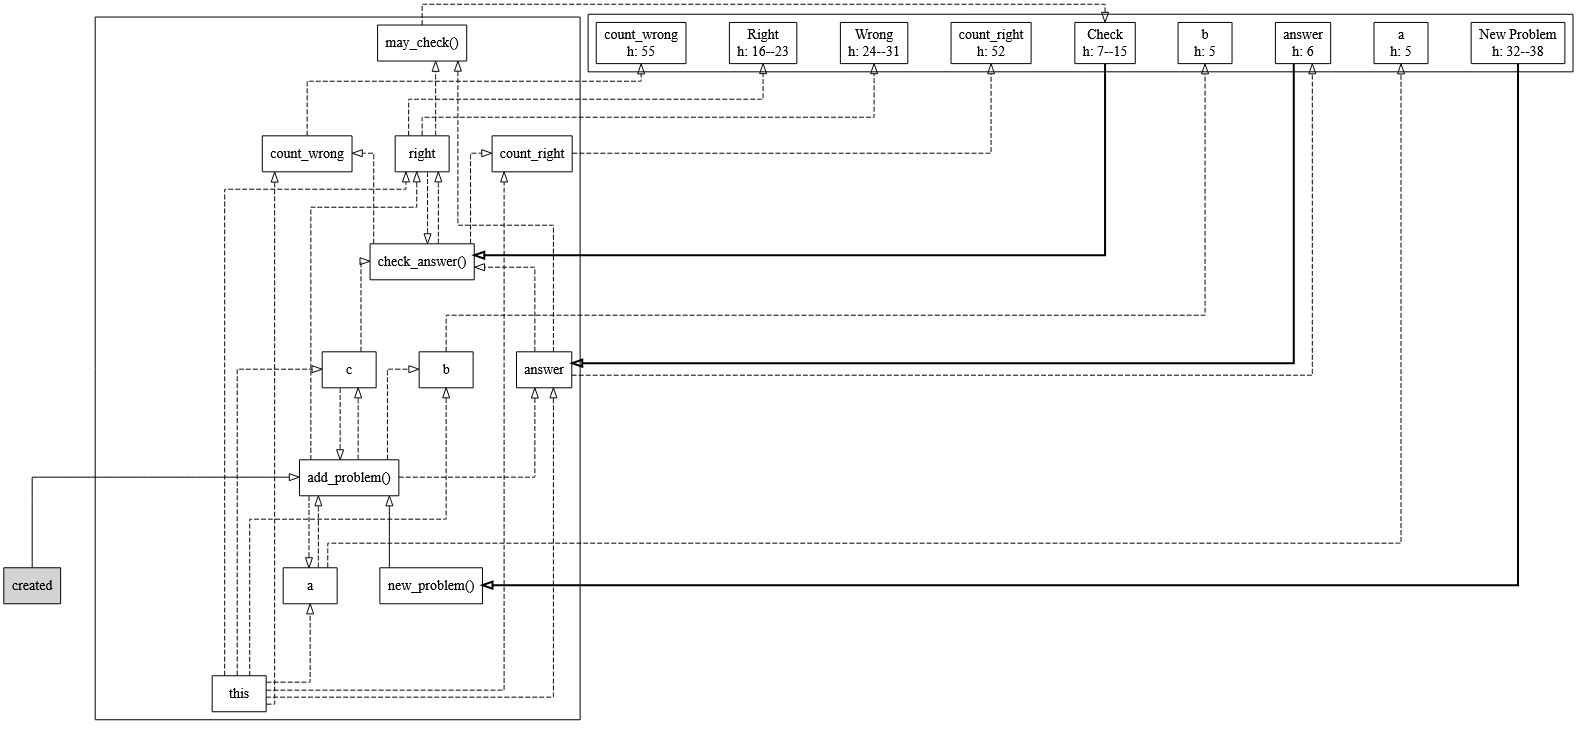
\includegraphics[width=\textwidth]{images/diagram_own_math_kids.png}
     \caption{Math for Kids in Vue.js generated interaction diagram }
     \label{fig:math_for_kids_own_interaction_diagram}
\end{figure}

\begin{figure}[H]
    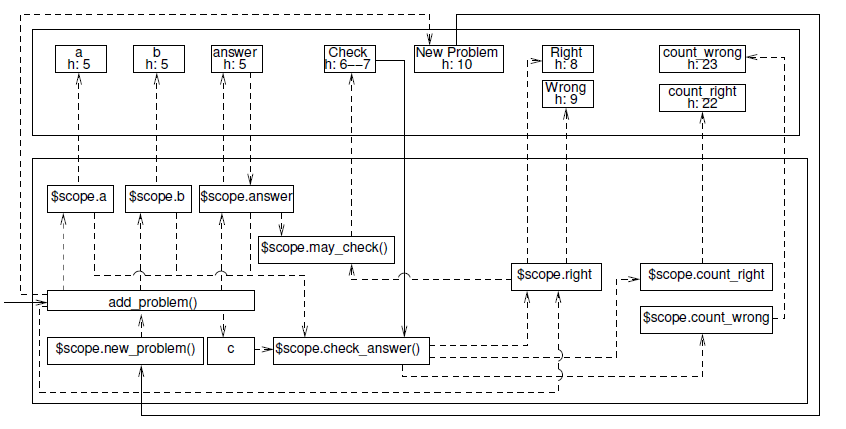
\includegraphics[width=\textwidth]{images/interaction_diagram_zhang.png}
     \caption{Math for Kids in AngularJS interaction diagram by \textcite{zhang2019scenario}}
     \label{fig:math_for_kids_zhang_interaction_diagram}
\end{figure}

When comparing the generated diagram\ref{fig:math_for_kids_own_interaction_diagram} to the original by \textcite{zhang2019scenario} \ref{fig:math_for_kids_zhang_interaction_diagram} there are some differences.

Due to different modelling there is a \code{this} vertex and connections from it to top level variables, which does not exist in the diagram by \textcite{zhang2019scenario}. In the generated diagram there is an edge of type 'event' between the \textit{answer} tag and \textit{answer} property. This is due to the way that two-way bindings were decided to be represented.

There are two differences between the \textit{add\_problem} node in the generated diagram and the one by \textit{zhang2019scenario}.
In \textcite{zhang2019scenario} there is an edge from
the \textit{add\_problem} method to the \textit{New Problem} tag, which is missing in the own generated version. This seems like a mistake in \parencite{zhang2019scenario}, since this edge should not exist.

The other difference is that in \parencite{zhang2019scenario} there is no edges from \textit{add\_problem} to \textit{right} (write relation), however there should be, 
inside \textit{add\_problem} \code{this.right = undefined}.

\begin{lstlisting}[language=JavaScript]
l(created) -> a, b, answer, Check, Right, Wrong
l(answer) -> answer, Check
l(Check) -> Right, Wrong, Check, count_right, count_wrong
l(New Problem) -> a, b, answer, Check, Right, Wrong
\end{lstlisting}

The generated reaction based on the graph differ for $l(created)$, all other sets are exactly the same as the ones by \textcite{zhang2019scenario} (albeit in different order). This may stem from the fact that the edges of \textit{add\_problem} to \code{\$scope.right} is missing in \parencite{zhang2019scenario}, however it is later correctly factored in $l(New Problem)$.

\textcite{zhang2019scenario} define $l(add_problem())$ 
(the equivalent of $l(created)$) as $l(add_problem() = 
{a, b})$ where it should be 
$l(add_problem() = {Check, Right, Wrong, a, b, answer })$ since the answer property is updated based on the diagram. 

One could argue, that the version in \parencite{zhang2019scenario} is correct, since $answer$ is set to $undefined$, which is the same as the initial value of the variable, so it would not trigger an update as part of the \code{init} method. The interaction diagram generator does not perform this check. If $l(add_problem())$ were to be called later in the application (when the $New Problem$ button is clicked) it would indeed set a new value to $answer$, which is correctly reflected by \textcite{zhang2019scenario}.


\subsection{Scenarios}
Gherkin scenarios of up to 4 actions are generated, which can be seen in the following figures. The program outputs the scenarios as plain text to the console, but here they are displayed in a nicer way. The caption of each figure is an example of how a text could be generated based on the template scenario output by the application.

Some scenarios seem a bit repetitive, but it is up to \textit{The Three Amigos} \ref{amigos} to decide which templates to discard. Since interaction diagrams model what \textit{might} be updated, it will probably be reasonable to discard some scenarios. The fact that everything which might get updated can also be leveraged in another way - negative criteria can be defined (assert tag/component $X$ did not change).
%TODO play around with subfigure alignment, there be
%https://tex.stackexchange.com/questions/333249/controlling-subfigure-captions-and-subfigure-placement
\begin{figure}[H]
    \caption{Gherkin scenarios templates and sample human written scenarios based on the templates }
    \centering
    \begin{subfigure}[b]{0.48\textwidth}
         \centering
         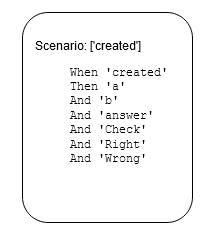
\includegraphics[width=0.48\textwidth]{images/scenarios_1.png}
         \caption{Scenario: initialization. When the application is created, then 'a' and 'b' should show random numbers and 'Check' should be disabled and 'Right' and Wrong should be invisible.}
    \end{subfigure}\hfill%
    \begin{subfigure}[b]{0.48\textwidth}
        \centering
        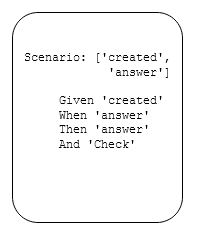
\includegraphics[width=0.48\textwidth]{images/scenarios_2.png}
        \caption{Scenario: typing an answer. Given the application has been created, when I type an answer then 'answer' should display it and 'Check' should be enabled.}
    \end{subfigure}\hfill%
    \begin{subfigure}[b]{0.48\textwidth}
        \centering
        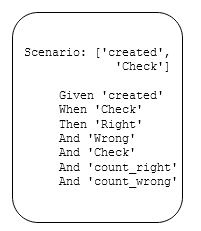
\includegraphics[width=0.48\textwidth]{images/scenarios_3.png}
        \caption{Scenario: clicking on check without typing an answer. Given the application has been created, when I click 'Check' then 'Right' and 'Wrong' should be invisible and 'count\_right' and 'count\_wrong' should have the same values and 'Check' should be disabled. }
   \end{subfigure}\hfill%
   \begin{subfigure}[b]{0.48\textwidth}
    \centering
    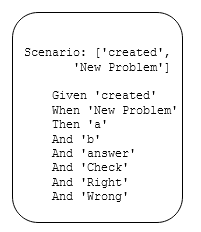
\includegraphics[width=0.48\textwidth]{images/scenarios_4.png}
    \caption{Scenario: obtaining a new problem at application start. Given the application has been created, when I click 'New Problem' then 'a' and 'b' should have random values and 'answer' should be empty and 'Check' should be disabled and 'Right' and 'Wrong' should be invisible.}
\end{subfigure}\hfill%
\end{figure}

\begin{figure}[H]\ContinuedFloat
    \centering

\begin{subfigure}[b]{0.48\textwidth}
    \centering
    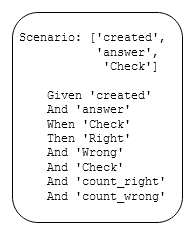
\includegraphics[width=0.48\textwidth]{images/scenarios_5.png}
    \caption{Scenario: checking my answer. Given the application has been created and 'answer' contains my answer, when I click 'Check' then 'Right' should be visible if the answer was right 'Wrong' should be visible if the answer was wrong and 'Check' should be disabled and 'count\_right' should be incremented by one if the answer was right and 'count\_wrong' should be incremented by one if the answer did not change. }
\end{subfigure}\hfill%
\begin{subfigure}[b]{0.48\textwidth}
    \centering
    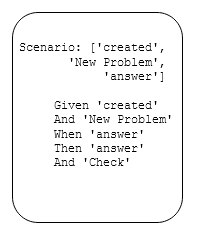
\includegraphics[width=0.48\textwidth]{images/scenarios_6.png}
    \caption{Scenario: typing an answer to a new problem. Given the application has been created and a new problem was obtained, when I type an answer then 'answer' should display it and 'Check' should be enabled.}
\end{subfigure}\hfill%
\begin{subfigure}[b]{0.48\textwidth}
    \centering
    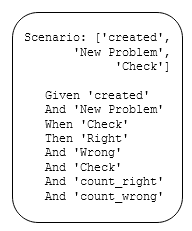
\includegraphics[width=0.48\textwidth]{images/scenarios_7.png}
    \caption{Scenario: requesting a new problem and clicking on check without answering it. Given the application has been created and I requested a new problem, when I click 'Check' then 'Right' and 'Wrong' should be invisible and 'count\_right' and 'count\_wrong' should have the same values and 'Check' should be disabled. }
\end{subfigure}\hfill%
\begin{subfigure}[b]{0.48\textwidth}
    \centering
    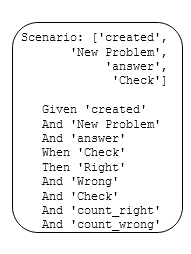
\includegraphics[width=0.48\textwidth]{images/scenarios_8.png}
    \caption{Scenario: requesting a new problem, answering it and checking my answer. Given the application has been created and I requested a new problem and answered it, when I click 'Check' then 'Right' should be visible if the answer was right 'Wrong' should be visible if the answer was wrong and 'Check' should be disabled and 'count\_right' should be incremented by one if the answer was right and 'count\_wrong' should be incremented by one if the answer did not change. }
\end{subfigure}

\end{figure}

\section{Math for Kids Extended - Lists and Computed Properties}

\ref{fig:eval_image_list_complex} shows an extension to the Math for Kids application. The full source code can be found it \ref{appendix:math_kids_extended_source_code}

The application now displays past problems in a list, randomly generates either a subtraction or addition problem, and also keeps tracks of statistics separated by problem type and includes and additional accuracy statistic.

\begin{figure}[H]
    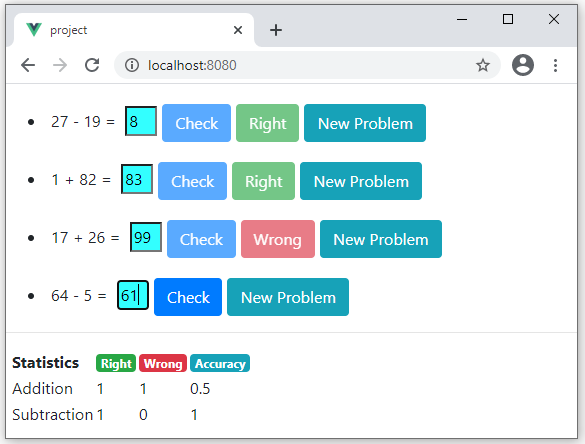
\includegraphics[width=\textwidth]{images/math_for_kids_own_complex.png}
     \caption{Math for Kids in Vue.js including subtraction problems, more precise statistics and display of past problems }
     \label{fig:eval_image_list_complex}
\end{figure}

\ref{fig:diagram_list_complex} shows the interaction diagram for the application, which looks more complex, but it is still possible to focus on specific components and see how they affect/are affected by others. 

The two vertices for the computed properties \textit{accuracy\_sub} and \textit{accuracy\_add} correctly directly depend on \textit{count\_right\_sub}, \textit{count\_wrong\_sub} and \textit{count\_right\_add}, \textit{count\_wrong\_add} respectively.

By looking at the reactions, one can observe that based on which of the mutually exclusive Check buttons is clicked on, either the substituting or addition related properties are updated. 

This example includes a bit of engineering - more realistically there would a single button, which checks inside the bound method which should be updated, however the application would not be able to be differentiate them in this case, since if statements inside methods are not supported.

This differentiation is also evident in the generated Gherkin scenario templates. 

All generated scenario templates up to 4 actions can be seen in  \ref{appendix:math_kids_extended_scenarios}

\begin{lstlisting}[language=JavaScript]
l(problems[i].answer) -> problems[i].answer, Check, Check
l(Check) -> Right, Wrong, Check, Check, count_right_add, accuracy_add, count_wrong_add
l(Check) -> Right, Wrong, Check, Check, count_right_sub, accuracy_sub, count_wrong_sub
l(New Problem) -> problems[i].a, +, -, Check, Check, problems[i].b, problems[i].answer, Right, Wrong
l(created) -> problems[i].a, +, -, Check, Check, problems[i].b, problems[i].answer, Right, Wrong
\end{lstlisting}

\begin{figure}[H]
    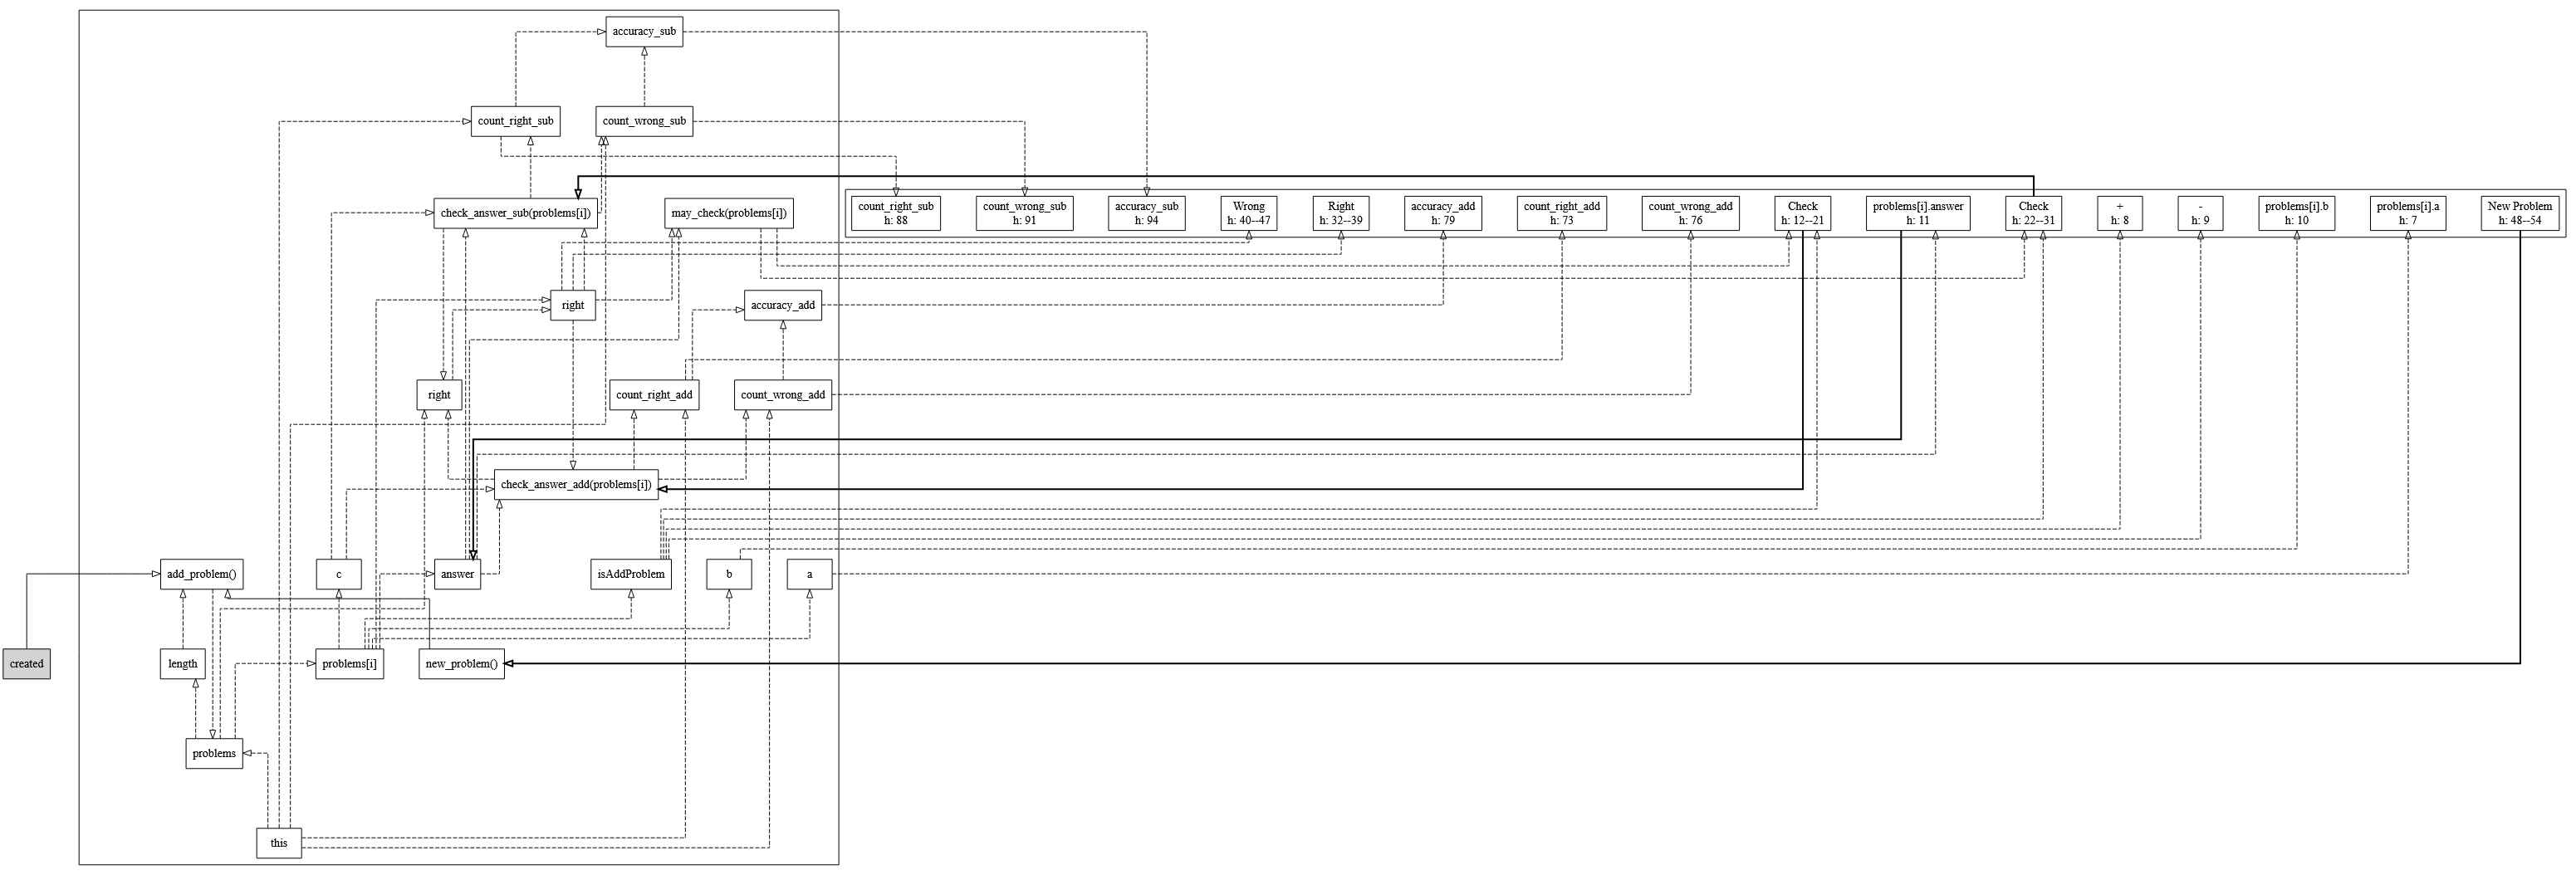
\includegraphics[width=\textwidth]{images/diagram_list_add_sub.png}
     \caption{Generated interaction diagram for Math for Kids including subtraction in Vue.js}
     \label{fig:diagram_list_complex}
\end{figure}



%TODO double check scenarios generated


\section{Daily Meals - Lists and Objects}

\ref{fig:eval_image_meal} shows a simple application, which displays a simplistic menu for a restaurant with a meal of the day. The full source code for it can be found in \ref{appendix:daily_menu_source_code}.

The daily meal and it's price is changed each day via a button click, and alternates between the first two items (the third item - steak is never the daily meal). There is also an option to discount the price of all items. Being the restaurants main source of income, there is also an additional advertisement label for steaks.
\begin{figure}[H]
    \centering
    \begin{subfigure}[b]{0.45\textwidth}
         \centering
         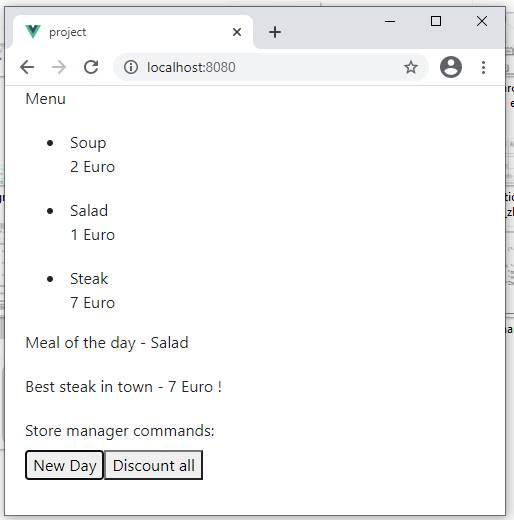
\includegraphics[width=0.45\textwidth]{images/meal_1.png}
         \caption{The current meal of the day is salad.}
    \end{subfigure}\hfill%
    \begin{subfigure}[b]{0.45\textwidth}
        \centering
        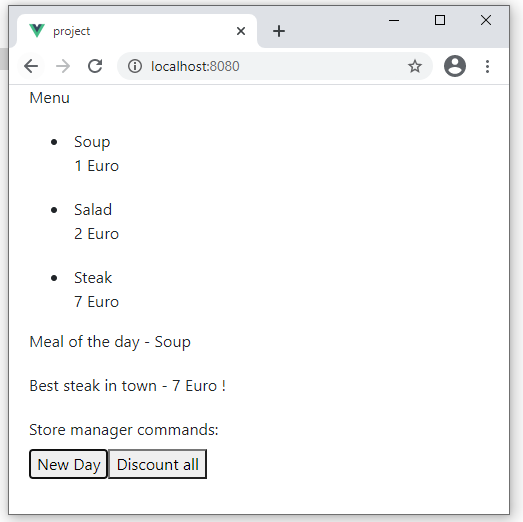
\includegraphics[width=0.45\textwidth]{images/meal_2.png}
        \caption{The 'new day' button has been clicked and the daily meal now changed to soup.}
    \end{subfigure}\hfill%
    \begin{subfigure}[b]{0.45\textwidth}
        \centering
        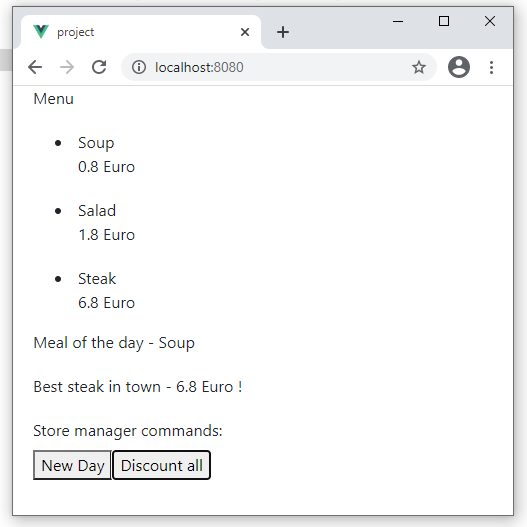
\includegraphics[width=0.45\textwidth]{images/meal_3.png}
        \caption{Discount was clicked and the price of all items got updated.}
    \end{subfigure}
    \caption{The menu with daily meal application }
    \label{fig:eval_image_meal}
\end{figure}

\ref{fig:diagram_meal_list_properties} shows the interaction diagram for the application and the resulting reactions and scenarios of up to 4 steps can be seen in \ref{eval:reactions_meal} and \ref{eval:scenarios_meal} respectively.

\label{eval:reactions_meal}
\begin{lstlisting}[language=JavaScript]
l(New Day) -> Price, Meal of the day -
l(Discount all) -> Best steak in town -, Price
l(created) -> meals[i].name, Price, Best steak in town -, Meal of the day -
\end{lstlisting}

As can be seen most clearly in \ref{eval:reactions_meal}, The 'New Day' button changes the 'Meal of the day' and some/all of the 'Price' list HTML tags. Only the price of each meal is changed, the 'meals[i].name' HTML tags remain the same. 'Best steak in town' is also not updated, since steak is never the daily meal. 

Clicking on 'Discount all' does indeed change both 'Best steak in town' and some/all 'Price' HTML tags, since everything is discounted.

\begin{figure}[H]
    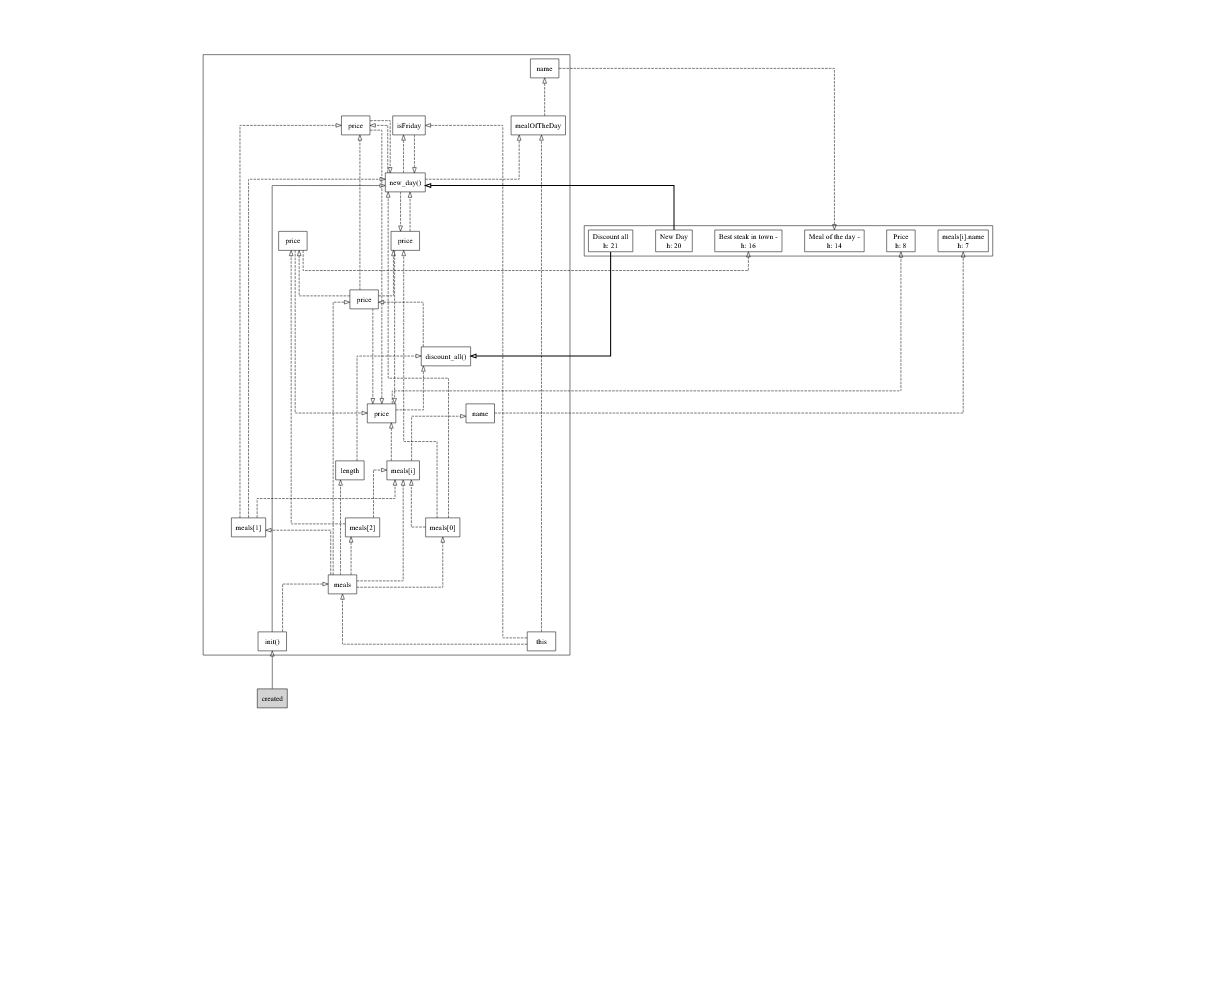
\includegraphics[width=\textwidth]{images/diagram_meal.png}
     \caption{Generated interaction diagram for Daily Menu}
     \label{fig:diagram_meal_list_properties}
\end{figure}

\label{eval:scenarios_meal}
\begin{lstlisting}[language=JavaScript]
Scenario: ['created']
	When 'created'
	Then 'meals[i].name'
	And 'Price'
	And 'Best steak in town -'
	And 'Meal of the day -'

Scenario: ['created', 'New Day']
	Given 'created'
	When 'New Day'
	Then 'Price'
	And 'Meal of the day -'

Scenario: ['created', 'Discount all']
	Given 'created'
	When 'Discount all'
	Then 'Best steak in town -'
	And 'Price'
\end{lstlisting}


\chapter{Conclusion}
\label{chapter:conclussion}
In this thesis an algorithm to generate interaction diagrams as described by \textcite{zhang2019scenario} for Vue.js was implemented and extended with support for lists objects and objects. Futher it was also shown how the interaction diagrams can be used to automatically generate Gherkin test scenario templates

The application is able to correctly generate interaction diagrams and scenario templates, which can be used to visualize the work flow of a \gls{spa}. The scenario tempaltes can successfully be used as an aid to generate very extensive Gherkin test scenarios. 


The application can be extended by more language constructs and features such as if-else statements, nested lists, arrow functions. In order to fully capture the complexity of JavaScript it must be extended to operate directly on a compelte \gls{ast}, such as the one generated by the ESLint parser.
A proper user interface for the Gherkin templates could also be implemented or it could be integrated as a plugin into existing Cucumber tools.

\newpage
\listoffigures{}

\lstlistoflistings

\printglossaries

%\listoftables{}

\nocite{*}
\printbibliography{}

\newpage
\appendix{}
\chapter{Appendix}
TODO code attached yada yada
\end{document}